\documentclass[thesis.tex]{subfiles}
\begin{document}
\selectlanguage{USenglish}
\chapter{Comparative Experimental Evaluation}
\label{ch:Results}

In this chapter we evaluate the performance of the new memetic algorithms by comparing them to state-of-the-art algorithms. In Section~\ref{sec:dimacs-results}, the results on the benchmark instances from the Second \gls{DIMACS} Implementation Challenge, which has been used as the training set for parameter tuning, are presented. The results on the validation instances are examined in Section~\ref{sec:validation-results}.


\section{Results on DIMACS Benchmark Instances}
%        ^^^^^^^^^^^^^^^^^^^^^^^^^^^^^^^^^^^^^
   \label{sec:dimacs-results}
   % BB-tw bachoore-bodlaender-2006-branchAndBound
   % QuickBB gogate-2004-quickbb
   % TabuTW clautiaux-2004-tabu
   % GAtw schafhauser-thesis,schafhauser-paper
   % IHA musliu-2008-ILS
   % ACS+ILS hammerl-thesis,hammerl-paper
%
   The benchmark instances of the Second \gls{DIMACS} Implementation Challenge are often used to judge the performance of treewidth heuristics. Consequently, we utilize them as well, in order to show how our memetic algorithms compare to state-of-the-art algorithms in the field:%
\begin{raggedright}
   \begin{itemize}\itemsep1ex
         \item Branch-and-bound algorithm for treewidth\\ by Bachoore and Bodlaender (BB-tw)~\parencite{bachoore-bodlaender-2006-branchAndBound}\glsunset{BBtw}
         \item Branch-and-bound algorithm for treewidth\\ by Gogate and Dechter (BB-tw)~\parencite{gogate-2004-quickbb}\glsunset{QuickBB}
         \item Tabu search for treewidth (TabuTW)~\parencite{clautiaux-2004-tabu}\glsunset{TabuTW}
         \item Ant colony system in combination with\\ iterated local search for treewidth (ACS+ILS)~\parencite{hammerl-thesis,hammerl-paper}\glsunset{ACSILS}
         \item Genetic algorithm for treewidth (GA-tw)~\parencite{schafhauser-thesis,schafhauser-paper}\glsunset{GA-tw}
         \item Iterative heuristic algorithm for treewidth (IHA)~\parencite{musliu-2008-ILS}\glsunset{IHA}
   \end{itemize}
\end{raggedright}
   
Please note that all involved algorithms have been tuned specifically for this instance set. Therefore, the results do not necessarily apply to other instances (see Section~\ref{sec:validation-results}).

   Using their original source code, the results for \gls{IHA} and \gls{GA-tw} have been gathered on the same platform and with the same time limit as for the memetic algorithms. However, the results for the other algorithms are presented using the measurements from their respective papers; they have been executed on different machines, using different running times. Consequently, the comparison has to be taken with a grain of salt in this regard. Note that also \gls{IHA} and \gls{GA-tw} improve some upper bounds with respect to what has been reported for them originally. This is due to a faster computing platform, compared to what was used for the original experiments.

   The algorithm runtime has been limited to one hour. For \gls{MA1}, \gls{MA2}, \gls{MA3}, \gls{IHA}, and \gls{GA-tw}, the given numbers represent the best upper bounds from 20 runs per algorithm and instance.

Table~\ref{tab:dimacs-results} displays the result. Upper bounds that are equal to the best result are typed in boldface. Improvements over the previously best known upper bounds are highlighted. It is shown that the memetic algorithms perform well, and are able to improve upper bounds for 8 instances.

The Table shows that \gls{MA3} achieves better results than \gls{TabuTW} and \gls{ACSILS} on many instances, although, as mentioned above, the results for the latter have been obtained using different hardware.

\gls{IHA} and \gls{GA-tw} both find good results for most instances. Additionally, we had access to their source code. Because of that, the experiments on the validation set were conducted using only these two heuristics as competitors to our approaches.

{\footnotesize
\begin{longtable}[c]{l S[table-format=3] S[table-format=6]%
                     S[table-format=3] S[table-format=3] S[table-format=3]%
                     S[table-format=3] S[table-format=3]
                     S[table-format=3] S[table-format=3] S[table-format=3] S[table-format=3]}
   \caption[Results on the benchmark instances of the\protect\newline Second DIMACS Implementation Challenge]{Results on the benchmark instances of the Second DIMACS Implementation Challenge}\label{tab:dimacs-results}\\ \toprule
   & \headeR{1}{l}{0}{$|V|$} & \headeR{1}{l}{0}{$|E|$} & \headeR{1}{l}{60}{\glsname{MA1}} & \headeR{1}{l}{60}{\glsname{MA2}} & \headeR{1}{l}{60}{\glsname{MA3}} & \headeR{1}{l}{60}{\glsname{IHA}} & \headeR{1}{l}{60}{\glsname{GA-tw}} & \headeR{1}{l}{60}{\glsname{TabuTW}} & \headeR{1}{l}{60}{\glsname{ACSILS}} & \headeR{1}{l}{60}{\glsname{BBtw}} & \headeR{1}{l}{60}{\glsname{QuickBB}} \\ \midrule\endfirsthead   \caption[]{(continued) Results on the benchmark instances of the Second DIMACS Implementation Challenge}\\ \toprule
   & \headeR{1}{l}{0}{$|V|$} & \headeR{1}{l}{0}{$|E|$} & \headeR{1}{l}{60}{\glsname{MA1}} & \headeR{1}{l}{60}{\glsname{MA2}} & \headeR{1}{l}{60}{\glsname{MA3}} & \headeR{1}{l}{60}{\glsname{IHA}} & \headeR{1}{l}{60}{\glsname{GA-tw}} & \headeR{1}{l}{60}{\glsname{TabuTW}} & \headeR{1}{l}{60}{\glsname{ACSILS}} & \headeR{1}{l}{60}{\glsname{BBtw}} & \headeR{1}{l}{60}{\glsname{QuickBB}} \\ \midrule\endhead
\Instance{myciel3} & 11 & 20 & \boldentry{3}{5} & \boldentry{3}{5} & \boldentry{3}{5} & \boldentry{3}{5} & \boldentry{3}{5} & \boldentry{3}{5} & \boldentry{3}{5} & \multicolumn{1}{c}{-} & \boldentry{3}{5}\\
\Instance{myciel4} & 23 & 71 & \boldentry{3}{10} & \boldentry{3}{10} & \boldentry{3}{10} & \boldentry{3}{10} & \boldentry{3}{10} & \boldentry{3}{10} & \boldentry{3}{10} & \multicolumn{1}{c}{-} & \boldentry{3}{10}\\
\Instance{queen5\textunderscore{}5} & 25 & 320 & \boldentry{3}{18} & \boldentry{3}{18} & \boldentry{3}{18} & \boldentry{3}{18} & \boldentry{3}{18} & \boldentry{3}{18} & \boldentry{3}{18} & \multicolumn{1}{c}{-} & \boldentry{3}{18}\\
\Instance{queen6\textunderscore{}6} & 36 & 580 & \boldentry{3}{25} & \boldentry{3}{25} & \boldentry{3}{25} & \boldentry{3}{25} & \boldentry{3}{25} & \boldentry{3}{25} & \boldentry{3}{25} & \multicolumn{1}{c}{-} & \boldentry{3}{25}\\
\Instance{myciel5} & 47 & 236 & \boldentry{3}{19} & \boldentry{3}{19} & \boldentry{3}{19} & \boldentry{3}{19} & \boldentry{3}{19} & \boldentry{3}{19} & \boldentry{3}{19} & \multicolumn{1}{c}{-} & \boldentry{3}{19}\\
\Instance{queen7\textunderscore{}7} & 49 & 952 & \boldentry{3}{35} & \boldentry{3}{35} & \boldentry{3}{35} & \boldentry{3}{35} & \boldentry{3}{35} & \boldentry{3}{35} & \boldentry{3}{35} & \multicolumn{1}{c}{-} & \boldentry{3}{35}\\
\Instance{queen8\textunderscore{}8} & 64 & 1456 & \boldentry{3}{45} & \boldentry{3}{45} & \boldentry{3}{45} & \boldentry{3}{45} & \boldentry{3}{45} & 46 & 46 & \multicolumn{1}{c}{-} & 46\\
\Instance{huck} & 74 & 602 & \boldentry{3}{10} & \boldentry{3}{10} & \boldentry{3}{10} & \boldentry{3}{10} & \boldentry{3}{10} & \boldentry{3}{10} & \boldentry{3}{10} & \multicolumn{1}{c}{-} & \boldentry{3}{10}\\
\Instance{jean} & 80 & 508 & \boldentry{3}{9} & \boldentry{3}{9} & \boldentry{3}{9} & \boldentry{3}{9} & \boldentry{3}{9} & \boldentry{3}{9} & \boldentry{3}{9} & \multicolumn{1}{c}{-} & \boldentry{3}{9}\\
\Instance{queen9\textunderscore{}9} & 81 & 2112 & \boldentry{3}{58} & \boldentry{3}{58} & \boldentry{3}{58} & \boldentry{3}{58} & \boldentry{3}{58} & \boldentry{3}{58} & 59 & \multicolumn{1}{c}{-} & 59\\
\Instance{david} & 87 & 812 & \boldentry{3}{13} & \boldentry{3}{13} & \boldentry{3}{13} & \boldentry{3}{13} & \boldentry{3}{13} & \boldentry{3}{13} & \boldentry{3}{13} & \boldentry{3}{13} & \boldentry{3}{13}\\
\Instance{myciel6} & 95 & 755 & \boldentry{3}{35} & \boldentry{3}{35} & \boldentry{3}{35} & \boldentry{3}{35} & \boldentry{3}{35} & \boldentry{3}{35} & \boldentry{3}{35} & \boldentry{3}{35} & \boldentry{3}{35}\\
\Instance{queen8\textunderscore{}12} & 96 & 2736 & \boldentry{3}{65} & \boldentry{3}{65} & \boldentry{3}{65} & \boldentry{3}{65} & \boldentry{3}{65} & \multicolumn{1}{c}{-} & \multicolumn{1}{c}{-} & \multicolumn{1}{c}{-} & \multicolumn{1}{c}{-}\\
\Instance{queen10\textunderscore{}10} & 100 & 2940 & \boldentry{3}{72} & \boldentry{3}{72} & \boldentry{3}{72} & \boldentry{3}{72} & \boldentry{3}{72} & \boldentry{3}{72} & 73 & \multicolumn{1}{c}{-} & \boldentry{3}{72}\\
\Instance{games120} & 120 & 1276 & 33 & \boldentry{3}{32} & \boldentry{3}{32} & \boldentry{3}{32} & \boldentry{3}{32} & 33 & 37 & 38 & \multicolumn{1}{c}{-}\\
\Instance{queen11\textunderscore{}11} & 121 & 3960 & \boldentry{3}{87} & \boldentry{3}{87} & \boldentry{3}{87} & \boldentry{3}{87} & \boldentry{3}{87} & 88 & 89 & \multicolumn{1}{c}{-} & 89\\
\Instance{DSJC125.1} & 125 & 1472 & 61 & \boldentry{3}{60} & \boldentry{3}{60} & \boldentry{3}{60} & \boldentry{3}{60} & 65 & 63 & 64 & 64\\
\Instance{DSJC125.5} & 125 & 7782 & \boldentry{3}{108} & \boldentry{3}{108} & \boldentry{3}{108} & \boldentry{3}{108} & \boldentry{3}{108} & 109 & \boldentry{3}{108} & 109 & 109\\
\Instance{DSJC125.9} & 125 & 13922 & \boldentry{3}{119} & \boldentry{3}{119} & \boldentry{3}{119} & \boldentry{3}{119} & \boldentry{3}{119} & \boldentry{3}{119} & \boldentry{3}{119} & \multicolumn{1}{c}{-} & \boldentry{3}{119}\\
\Instance{miles1000} & 128 & 6432 & \boldentry{3}{49} & \boldentry{3}{49} & \boldentry{3}{49} & \boldentry{3}{49} & \boldentry{3}{49} & \boldentry{3}{49} & 50 & \multicolumn{1}{c}{-} & \boldentry{3}{49}\\
\Instance{miles1500} & 128 & 10396 & \boldentry{3}{77} & \boldentry{3}{77} & \boldentry{3}{77} & \boldentry{3}{77} & \boldentry{3}{77} & \boldentry{3}{77} & \boldentry{3}{77} & \multicolumn{1}{c}{-} & \boldentry{3}{77}\\
\Instance{miles250} & 128 & 774 & \boldentry{3}{9} & \boldentry{3}{9} & \boldentry{3}{9} & \boldentry{3}{9} & 10 & \boldentry{3}{9} & \boldentry{3}{9} & \multicolumn{1}{c}{-} & \boldentry{3}{9}\\
\Instance{miles500} & 128 & 2340 & 24 & 23 & \boldentry{3}{22} & \boldentry{3}{22} & 24 & \boldentry{3}{22} & 25 & \multicolumn{1}{c}{-} & \boldentry{3}{22}\\
\Instance{miles750} & 128 & 4226 & 37 & \boldentry{3}{36} & \boldentry{3}{36} & \boldentry{3}{36} & 37 & \boldentry{3}{36} & 38 & \multicolumn{1}{c}{-} & 37\\
\Instance{anna} & 138 & 986 & \boldentry{3}{12} & \boldentry{3}{12} & \boldentry{3}{12} & \boldentry{3}{12} & \boldentry{3}{12} & \boldentry{3}{12} & \boldentry{3}{12} & \boldentry{3}{12} & \boldentry{3}{12}\\
\Instance{queen12\textunderscore{}12} & 144 & 5192 & 104 & \boldentry{3}{103} & \boldentry{3}{103} & \boldentry{3}{103} & 104 & 104 & 109 & \multicolumn{1}{c}{-} & 110\\
\Instance{queen13\textunderscore{}13} & 169 & 6656 & 122 & \boldentry{3}{121} & 122 & \boldentry{3}{121} & \boldentry{3}{121} & 122 & 128 & \multicolumn{1}{c}{-} & 125\\
\Instance{mulsol.i.3} & 184 & 3916 & \boldentry{3}{32} & \boldentry{3}{32} & \boldentry{3}{32} & \boldentry{3}{32} & \boldentry{3}{32} & \boldentry{3}{32} & \boldentry{3}{32} & \multicolumn{1}{c}{-} & \boldentry{3}{32}\\
\Instance{mulsol.i.4} & 185 & 3946 & \boldentry{3}{32} & \boldentry{3}{32} & \boldentry{3}{32} & \boldentry{3}{32} & \boldentry{3}{32} & \boldentry{3}{32} & \boldentry{3}{32} & \multicolumn{1}{c}{-} & \boldentry{3}{32}\\
\Instance{mulsol.i.5} & 186 & 3973 & \boldentry{3}{31} & \boldentry{3}{31} & \boldentry{3}{31} & \boldentry{3}{31} & \boldentry{3}{31} & \boldentry{3}{31} & \boldentry{3}{31} & \multicolumn{1}{c}{-} & \boldentry{3}{31}\\
\Instance{mulsol.i.2} & 188 & 3885 & \boldentry{3}{32} & \boldentry{3}{32} & \boldentry{3}{32} & \boldentry{3}{32} & \boldentry{3}{32} & \boldentry{3}{32} & \boldentry{3}{32} & \multicolumn{1}{c}{-} & \boldentry{3}{32}\\
\Instance{myciel7} & 191 & 2360 & 66 & 66 & 66 & 66 & 66 & 66 & 66 & 66 & \boldentry{3}{54}\\
\Instance{queen14\textunderscore{}14} & 196 & 8372 & 142 & 141 & 142 & \boldentry{3}{140} & \boldentry{3}{140} & 141 & 150 & \multicolumn{1}{c}{-} & 143\\
\Instance{mulsol.i.1} & 197 & 3925 & \boldentry{3}{50} & \boldentry{3}{50} & \boldentry{3}{50} & \boldentry{3}{50} & \boldentry{3}{50} & \boldentry{3}{50} & \boldentry{3}{50} & \multicolumn{1}{c}{-} & \boldentry{3}{50}\\
\Instance{zeroin.i.3} & 206 & 3540 & \boldentry{3}{32} & \boldentry{3}{32} & \boldentry{3}{32} & \boldentry{3}{32} & \boldentry{3}{32} & \boldentry{3}{32} & 33 & \multicolumn{1}{c}{-} & \multicolumn{1}{c}{-}\\
\Instance{zeroin.i.1} & 211 & 4100 & \boldentry{3}{50} & \boldentry{3}{50} & \boldentry{3}{50} & \boldentry{3}{50} & \boldentry{3}{50} & \boldentry{3}{50} & \boldentry{3}{50} & \multicolumn{1}{c}{-} & \multicolumn{1}{c}{-}\\
\Instance{zeroin.i.2} & 211 & 3541 & \boldentry{3}{32} & \boldentry{3}{32} & \boldentry{3}{32} & \boldentry{3}{32} & \boldentry{3}{32} & \boldentry{3}{32} & 33 & \multicolumn{1}{c}{-} & \multicolumn{1}{c}{-}\\
\Instance{queen15\textunderscore{}15} & 225 & 10360 & 164 & 162 & \boldentry{3}{\cellcolor{GreenYellow}161} & 162 & \boldentry{3}{\cellcolor{GreenYellow}161} & 163 & 174 & \multicolumn{1}{c}{-} & 167\\
\Instance{DSJC250.1} & 250 & 6436 & 173 & 170 & 168 & \boldentry{3}{167} & \boldentry{3}{167} & 173 & 174 & 177 & 176\\
\Instance{DSJC250.5} & 250 & 31336 & 230 & 230 & 230 & \boldentry{3}{229} & 230 & 232 & 231 & \multicolumn{1}{c}{-} & 231\\
\Instance{DSJC250.9} & 250 & 55794 & \boldentry{3}{243} & \boldentry{3}{243} & \boldentry{3}{243} & \boldentry{3}{243} & \boldentry{3}{243} & \boldentry{3}{243} & \boldentry{3}{243} & \multicolumn{1}{c}{-} & \boldentry{3}{243}\\
\Instance{queen16\textunderscore{}16} & 256 & 12640 & 187 & 184 & \boldentry{3}{\cellcolor{GreenYellow}183} & 184 & 185 & 186 & 201 & \multicolumn{1}{c}{-} & 205\\
\Instance{flat300\textunderscore{}20\textunderscore{}0} & 300 & 21375 & 278 & 278 & 279 & \boldentry{3}{277} & 278 & \multicolumn{1}{c}{-} & \multicolumn{1}{c}{-} & \multicolumn{1}{c}{-} & \multicolumn{1}{c}{-}\\
\Instance{flat300\textunderscore{}26\textunderscore{}0} & 300 & 21633 & 279 & 278 & 278 & \boldentry{3}{277} & 279 & \multicolumn{1}{c}{-} & \multicolumn{1}{c}{-} & \multicolumn{1}{c}{-} & \multicolumn{1}{c}{-}\\
\Instance{flat300\textunderscore{}28\textunderscore{}0} & 300 & 21695 & 279 & 279 & 279 & \boldentry{3}{278} & 279 & \multicolumn{1}{c}{-} & \multicolumn{1}{c}{-} & \multicolumn{1}{c}{-} & \multicolumn{1}{c}{-}\\
\Instance{school1\textunderscore{}nsh} & 352 & 14612 & 159 & 153 & \boldentry{3}{\cellcolor{GreenYellow}151} & 152 & 156 & 162 & 185 & \multicolumn{1}{c}{-} & \multicolumn{1}{c}{-}\\
\Instance{school1} & 385 & 19095 & 190 & 179 & \boldentry{3}{\cellcolor{GreenYellow}176} & 178 & 182 & 188 & 228 & 178 & \multicolumn{1}{c}{-}\\
\Instance{fpsol2.i.3} & 425 & 8688 & 32 & \boldentry{3}{31} & \boldentry{3}{31} & \boldentry{3}{31} & \boldentry{3}{31} & \boldentry{3}{31} & \boldentry{3}{31} & \multicolumn{1}{c}{-} & \boldentry{3}{31}\\
\Instance{le450\textunderscore{}15a} & 450 & 8168 & 278 & 263 & 259 & 259 & \boldentry{3}{\cellcolor{GreenYellow}258} & 272 & 288 & \multicolumn{1}{c}{-} & \multicolumn{1}{c}{-}\\
\Instance{le450\textunderscore{}15b} & 450 & 8169 & 275 & 264 & 262 & \boldentry{3}{258} & 264 & 270 & 292 & \multicolumn{1}{c}{-} & 289\\
\Instance{le450\textunderscore{}15c} & 450 & 16680 & 362 & 355 & 351 & 351 & \boldentry{3}{\cellcolor{GreenYellow}349} & 359 & 368 & \multicolumn{1}{c}{-} & 372\\
\Instance{le450\textunderscore{}15d} & 450 & 16750 & 365 & 355 & 352 & \boldentry{3}{\cellcolor{GreenYellow}351} & 353 & 360 & 371 & \multicolumn{1}{c}{-} & 371\\
\Instance{le450\textunderscore{}25a} & 450 & 8260 & 233 & 221 & 220 & \boldentry{3}{216} & 225 & 234 & 249 & \multicolumn{1}{c}{-} & 255\\
\Instance{le450\textunderscore{}25b} & 450 & 8263 & 231 & 216 & \boldentry{3}{\cellcolor{GreenYellow}211} & 214 & 222 & 233 & 245 & \multicolumn{1}{c}{-} & 251\\
\Instance{le450\textunderscore{}25c} & 450 & 17343 & 334 & 323 & \boldentry{3}{320} & 322 & \boldentry{3}{320} & 327 & 346 & \multicolumn{1}{c}{-} & 349\\
\Instance{le450\textunderscore{}25d} & 450 & 17425 & 336 & 330 & \boldentry{3}{\cellcolor{GreenYellow}325} & 326 & 326 & 336 & 355 & \multicolumn{1}{c}{-} & 349\\
\Instance{le450\textunderscore{}5a} & 450 & 5714 & 263 & 247 & 244 & 245 & \boldentry{3}{243} & 256 & 304 & 304 & 307\\
\Instance{le450\textunderscore{}5b} & 450 & 5734 & 256 & 248 & \boldentry{3}{246} & \boldentry{3}{246} & 247 & 254 & 308 & \multicolumn{1}{c}{-} & 309\\
\Instance{le450\textunderscore{}5c} & 450 & 9803 & 272 & 265 & \boldentry{3}{\cellcolor{GreenYellow}263} & 265 & 264 & 272 & 309 & \multicolumn{1}{c}{-} & 315\\
\Instance{le450\textunderscore{}5d} & 450 & 9757 & 269 & 263 & \boldentry{3}{\cellcolor{GreenYellow}262} & 265 & 265 & 278 & 290 & \multicolumn{1}{c}{-} & 303\\
\Instance{fpsol2.i.2} & 451 & 8691 & 32 & 32 & \boldentry{3}{31} & \boldentry{3}{31} & \boldentry{3}{31} & \boldentry{3}{31} & \boldentry{3}{31} & \multicolumn{1}{c}{-} & \boldentry{3}{31}\\
\Instance{fpsol2.i.1} & 496 & 11654 & \boldentry{3}{66} & \boldentry{3}{66} & \boldentry{3}{66} & \boldentry{3}{66} & \boldentry{3}{66} & \boldentry{3}{66} & \boldentry{3}{66} & \multicolumn{1}{c}{-} & \boldentry{3}{66}\\
\Instance{DSJC500.1} & 500 & 24916 & 410 & 401 & 396 & 396 & \boldentry{3}{\cellcolor{GreenYellow}395} & \multicolumn{1}{c}{-} & \multicolumn{1}{c}{-} & \multicolumn{1}{c}{-} & 409\\
\Instance{DSJC500.5} & 500 & 125248 & \boldentry{3}{\cellcolor{GreenYellow}477} & 478 & \boldentry{3}{\cellcolor{GreenYellow}477} & \boldentry{3}{\cellcolor{GreenYellow}477} & \boldentry{3}{\cellcolor{GreenYellow}477} & \multicolumn{1}{c}{-} & \multicolumn{1}{c}{-} & \multicolumn{1}{c}{-} & 479\\
\Instance{DSJC500.9} & 500 & 224874 & \boldentry{3}{492} & \boldentry{3}{492} & \boldentry{3}{492} & \boldentry{3}{492} & \boldentry{3}{492} & \multicolumn{1}{c}{-} & \multicolumn{1}{c}{-} & \multicolumn{1}{c}{-} & \boldentry{3}{492}\\
\Instance{DSJR500.1} & 500 & 7110 & 43 & 35 & \boldentry{3}{33} & 35 & 34 & \multicolumn{1}{c}{-} & \multicolumn{1}{c}{-} & \multicolumn{1}{c}{-} & \multicolumn{1}{c}{-}\\
\Instance{DSJR500.1c} & 500 & 242550 & \boldentry{3}{485} & \boldentry{3}{485} & \boldentry{3}{485} & \boldentry{3}{485} & \boldentry{3}{485} & \multicolumn{1}{c}{-} & \multicolumn{1}{c}{-} & \multicolumn{1}{c}{-} & \boldentry{3}{485}\\
\Instance{DSJR500.5} & 500 & 117724 & 263 & 250 & 246 & 250 & 258 & \multicolumn{1}{c}{-} & \multicolumn{1}{c}{-} & \multicolumn{1}{c}{-} & \boldentry{3}{175}\\
\Instance{homer} & 561 & 3258 & 29 & \boldentry{3}{\cellcolor{GreenYellow}27} & \boldentry{3}{\cellcolor{GreenYellow}27} & 31 & 31 & 31 & 30 & \multicolumn{1}{c}{-} & 31\\
\Instance{inithx.i.3} & 621 & 13969 & 35 & 35 & 35 & 35 & 35 & 35 & \boldentry{3}{31} & 35 & \boldentry{3}{31}\\
\Instance{inithx.i.2} & 645 & 13979 & 35 & 35 & 35 & 35 & 35 & 35 & \boldentry{3}{31} & 35 & \boldentry{3}{31}\\
\Instance{inithx.i.1} & 864 & 18707 & \boldentry{3}{56} & \boldentry{3}{56} & \boldentry{3}{56} & \boldentry{3}{56} & \boldentry{3}{56} & \boldentry{3}{56} & \boldentry{3}{56} & \multicolumn{1}{c}{-} & \boldentry{3}{56}\\
\Instance{latin\footnote{\Instance{latin\textunderscore{}square\textunderscore{}10}}} & 900 & 307350 & \boldentry{3}{851} & \boldentry{3}{851} & \boldentry{3}{851} & \boldentry{3}{851} & \boldentry{3}{851} & \multicolumn{1}{c}{-} & \multicolumn{1}{c}{-} & \multicolumn{1}{c}{-} & \multicolumn{1}{c}{-}\\
\Instance{DSJC1000.1} & 1000 & 99258 & 901 & 891 & 882 & 882 & \boldentry{3}{\cellcolor{GreenYellow}874} & \multicolumn{1}{c}{-} & \multicolumn{1}{c}{-} & \multicolumn{1}{c}{-} & 896\\
\Instance{DSJC1000.5} & 1000 & 499652 & 978 & 975 & 976 & \boldentry{3}{\cellcolor{GreenYellow}974} & 975 & \multicolumn{1}{c}{-} & \multicolumn{1}{c}{-} & \multicolumn{1}{c}{-} & 977\\
\Instance{DSJC1000.9} & 1000 & 898898 & \boldentry{3}{991} & 992 & 992 & \boldentry{3}{991} & 992 & \multicolumn{1}{c}{-} & \multicolumn{1}{c}{-} & \multicolumn{1}{c}{-} & \boldentry{3}{991}\\
\Instance{flat1000\textunderscore{}50\textunderscore{}0} & 1000 & 245000 & 978 & 976 & 975 & \boldentry{3}{974} & 975 & \multicolumn{1}{c}{-} & \multicolumn{1}{c}{-} & \multicolumn{1}{c}{-} & \multicolumn{1}{c}{-}\\
\Instance{flat1000\textunderscore{}60\textunderscore{}0} & 1000 & 245830 & 978 & 976 & 976 & \boldentry{3}{975} & \boldentry{3}{975} & \multicolumn{1}{c}{-} & \multicolumn{1}{c}{-} & \multicolumn{1}{c}{-} & \multicolumn{1}{c}{-}\\
\Instance{flat1000\textunderscore{}76\textunderscore{}0} & 1000 & 246708 & 978 & 976 & 976 & \boldentry{3}{974} & 975 & \multicolumn{1}{c}{-} & \multicolumn{1}{c}{-} & \multicolumn{1}{c}{-} & \multicolumn{1}{c}{-}\\
   \bottomrule
\end{longtable}}



\section{Algorithm Validation}
%        ^^^^^^^^^^^^^^^^^^^^
   \label{sec:validation-results}
%
The algorithms are validated on a set of instances that is deliberately distinct from the training set used in the previous chapter. This validation set, which is listed in Tables~\vref{validationset1} and~\vref{validationset2}, has been taken from TreewidthLib~\parencite{treewidthlib}, a website devoted to treewidth benchmark instances (and algorithms), created by Jan-Willem van den Broek and Hans Bodlaender. Using two distinct sets of instances ensures that we are able to improve best known upper bounds on the training instances by specifically tuning for them, and, at the same time, reason about the universal performance of the algorithms.

\newlength{\RowSeparatorLength}
\setlength{\RowSeparatorLength}{.4\baselineskip}
\begin{table}[tbp]
   %\begin{sidefigure}{toc={Instances 1--12 of the validation set},caption={The validation set, instances 1--12. The instance files and the corresponding descriptions have been taken from~\parencite{treewidthlib}},label=validationset1,place=tbp}
   \caption[Instances 1--12 of the validation set]{The validation set, instances 1--12. The instance files and the corresponding descriptions have been taken from~\parencite{treewidthlib}}
   \label{validationset1}
   \centering\footnotesize
   \begin{tabularx}{\textwidth}{p{5em}S[table-format=4]S[table-format=4]>{\raggedright\arraybackslash}X} \toprule
      %\multicolumn{4}{c}{\header{Validation Set, Instances 1--12}} \\
      & \header{|V|} & \header{|E|} & \\\midrule

      \Instance{barley} & 48 & 126 &
      The first version of the Barley network, a probabilistic network developed by Kristensen and Rasmussen in a project for growing malting barley without use of pesticides. This is the moralized graph of the network.\\[\RowSeparatorLength]

      \Instance{rl5934}  & 2048 & 3087 &
      %\multirow{4}{28em}[\baselineskip]{TSP Graphs from the work of Cook and Seymour.}\\
      \multirow{4}{28em}{TSP Graphs from the work of Cook and Seymour.}\\
      \Instance{pcb3038} & 1985 & 3109 & \\
      \Instance{fnl4461} & 3326 & 5147 & \\
      \Instance{fl3795}  & 2103 & 3973 & \\[\RowSeparatorLength]

      \Instance{pathfinder} & 109 & 211 &
      A probabilistic network for assisting surgical pathologists with the diagnosis of lymph-node diseases. The graph given here is the undirected graph, obtained from applying moralization to the directed probabilistic network.\\[\RowSeparatorLength]

      \Instance{oesoca+} & 67 & 208 &
      Probabilistic network for staging of oesophageal carcinoma, developed at Utrecht University by L.\@ van der Gaag et al. The graph given here is the version after the moralization step.\\[\RowSeparatorLength]

      \Instance{link} & 724 & 1738 &
      Probabilistic network for linkage analysis.\\[\RowSeparatorLength]

      \Instance{diabetes} & 413 & 819 &
      A preliminary model for insulin dose adjustment that consists of 24 structurally identical subnetworks interconnected via temporal links.~\parencite{DiabetesInstances}
      \\[\RowSeparatorLength]

      \Instance{pigs} & 441 & 806 &
      Pedigree of breeding pigs. The pedigree is used for diagnosing the PSE disease. Created by Claus S.\@ Jensen on the basis of a data base from Søren Andersen (Danske Slagterier, Axeltorv Copenhagen).
      \\[\RowSeparatorLength]

      \Instance{water} & 32 & 123 &
      Preliminary model of the biological processes of a water purificationplant. The network consists of four structurally identical subnetworks, each representing a time slice of 15 minutes. The network was developedby Finn V.\@ Jensen, Uffe Kjærulff, Kristian G.\@ Olesen, and Jan Pedersen. This is a probabilistic network, given here after the moralization step.
      \\[\RowSeparatorLength]

      \Instance{munin1} & 189 & 366 &
      A subset of the Munin network; a probablistic network. The version here is after the moralization step.\\
   \bottomrule
   \end{tabularx}
\end{table}
\begin{table}[htbp]
   %\begin{sidefigure}{toc={Instances 13--27 of the validation set},caption={The validation set, instances 13--27. The instance files and the corresponding descriptions have been taken from~\parencite{treewidthlib}},label=validationset2,place=tbp}
   \caption[Instances 13--27 of the validation set]{The validation set, instances 13--27. The instance files and the corresponding descriptions have been taken from~\parencite{treewidthlib}}
   \label{validationset2}
   \centering\footnotesize
   \begin{tabularx}{\textwidth}{p{5em}S[table-format=4]S[table-format=4]>{\raggedright\arraybackslash}X} \toprule
      %\multicolumn{4}{c}{\header{Validation Set, Instances 13--27}} \\
      & \header{|V|} & \header{|E|} & \\\midrule

      \Instance{1ubq} & 74 & 211 &
      A graph from the field of computational biology, where tree decomposition directs a dynamic programming algorithm for protein redesign. The graph comes from ubiquitin, a well studied protein (PDB ID 1ubq). Each vertex represents a single side chain. Each edge represents the existence of a pairwise interaction between the two side chains. Copyright Andrew Leaver-Fay.\\[\RowSeparatorLength]

      \Instance{knights8\textunderscore{}8} & 64 & 168 &
      The vertices of this graph correspond to the squares of an 8 by 8 chessboard. There is an edge between vertices if these are a knights-move away from each other. The origin of this graph can be found in the more than 1000 years old knights-tour puzzle: to find a Hamiltonian path or cycle in this graph.\\[\RowSeparatorLength]

      \Instance{1a62} & 122 & 1516 & 
      \multirow{7}{28em}{A graphs from the field of computational biology, where tree decomposition directs a dynamic programming algorithm for protein redesign. Each vertex represents a single side chain. Each edge represents the existence of a pairwise interaction between the two side chains. Copyright Andrew Leaver-Fay.}\\
      \Instance{1sem} &  57 &  570 & \\
      \Instance{1qtn} &  87 &  788 & \\
      \Instance{1pwt} &  61 &  657 & \\
      \Instance{1or7} & 180 & 1875 & \\
      \Instance{1on2} & 135 & 1527 & \\
      \Instance{1oai} &  58 &  524 & \\[\RowSeparatorLength]
      
      \Instance{BN\textunderscore{}0} & 100 & 300 &
      Moralized version of a graph used in the UAI 2006 Inference Evaluation. This is a random modification of the Alarm network.\\[\RowSeparatorLength]

      \Instance{BN\textunderscore{}16} & 2127 & 5581 &
      Moralized version of a graph used in the UAI 2006 Inference Evaluation. This is a modified form of the Diagnosis graph.\\[\RowSeparatorLength]

      \Instance{BN\textunderscore{}20} & 2843 & 8108 &
      Moralized version of a graph used in the UAI 2006 Inference Evaluation. This is a DBN from speech recognition that is unrolled a fixed amount.\\[\RowSeparatorLength]

      \Instance{BN\textunderscore{}30} & 1156 & 3333 &
      Moralized version of a DAG used in the UAI 2006 Inference Evaluation. The original DAG was a grid.\\[\RowSeparatorLength]

      \Instance{BN\textunderscore{}42} & 880 & 1577 &
      Moralized version of a DAG used in the UAI 2006 Inference Evaluation. The original DAG was from iscas85.\\[\RowSeparatorLength]

      \Instance{BN\textunderscore{}47} & 661 & 2131 &
      Moralized version of a DAG used in the UAI 2006 Inference Evaluation. The original DAG was from iscas89.\\
   \bottomrule
   \end{tabularx}
\end{table}

The validation runs for \gls{GA-tw} and \gls{IHA} have been executed with their respective original implementation. Merely minor modification have been applied, which were required for compilation and solution extraction.
%They are shown as patches in Git format in Chapter~\vref{ch:patches}. 
%They may be examined using the source directory (there the two helper scripts \verb|get_GAtw_diff.sh| and \verb|get_IHA_diff.sh| are provided in the project's root directory).

By using the exact same instances for all involved algorithms, instance variability is factored out of the comparison~\parencite{theoreticians-guide-to-experimental-analysis} (this method is also known as \textit{blocking on instances}~\parencite{experimental-tutorial}).

Due to the architectural differences in the algorithms, there is no natural metric for measuring their progress. Instead, a limit on their runtime is imposed. We chose a limit of one hour, which seems reasonable, considering that the involved algorithms are usually meant for preprocessing a problem instance before handing over the result to another algorithm that actually solves the original problem. By forbearing from longer running times, we were able to gather 20 samples for each of the 5 validated algorithms, for each of the 106 instances (that includes the runs for Section~\ref{sec:dimacs-results}), in a time of 10600 hours, or approximately 442 days. In other words, the one hour runtime limit and the sample size of 20 represent a compromise between the time needed for the validation, and its informative value.

\clearpage
The experiments have been done on an AMD Opteron 6272 CPU, running at 2.1\,GHz, with access to roughly 220\,GB of memory. Since the CPU speed is the most important performance factor for this work's heuristic algorithms, the following result of the (randomly selected) \emph{pystone} benchmark may be taken into consideration when reproducing the presented results:
\begin{center}
\begin{verbatim}
$ python2 --version
Python 2.7.3
$ python2 -c "from test import pystone; pystone.main()"
Pystone(1.1) time for 50000 passes = 0.71
This machine benchmarks at 70422.5 pystones/second
\end{verbatim}
\end{center}


\subsection{Results}
%        ^^^^^^^^^^^^^^^^^^^^^^^^^^^^^^^^^^^^
   \label{sec:validation-performance}
%
\sisetup{%
   add-decimal-zero=true,
   add-integer-zero=false,
   round-mode=off,
   %round-precision=1,
   separate-uncertainty=true,
}
\newcommand{\CurrentInstanceOrig}{}
\newcommand{\CurrentInstance}{}
\newcommand{\CurrentInstanceFileEscaped}{}
\newcommand{\CurrentInstanceTexEscaped}{}

In the following the results for the validation set are presented. Those instances on which all tested algorithms perform very similarly are listed in Chapter~\vref{appendix:boring-validation-instances}.
%To be space efficient, we show some plots only for arbitrarily selected instances, which represent two small, two medium sized, and two large instances.

% ---------------------------------------------------------------------------- %
\subsubsection{\Instance{rl5934}}
   \renewcommand{\CurrentInstance}{\Instance{rl5934}}
   \renewcommand{\CurrentInstanceFileEscaped}{rl5934}
   \renewcommand{\CurrentInstanceTexEscaped}{rl5934}
\input{generated-tables/validation-validationset-\CurrentInstanceFileEscaped-results.tex}
\begin{figure}[hbtp]
   \centering
   \includegraphics[width=.65\textwidth]{plots/validation-validationset-\CurrentInstanceFileEscaped-violin.pdf}
   \caption{Violin plot for instance \CurrentInstance}
   \label{fig:\CurrentInstanceFileEscaped-violin}
\end{figure}
%\begin{sidefigure}{caption={Violin plot for instance \CurrentInstance},label={fig:\CurrentInstanceFileEscaped-violin},place={htbp}}
   %\includegraphics[width=.7\textwidth]{plots/validation-validationset-\CurrentInstanceFileEscaped-violin.pdf}
%\end{sidefigure}


\begin{figure}[hbtp]
   \centering
   \includegraphics[width=\textwidth]{plots/validation-validationset-\CurrentInstanceFileEscaped-timings-crop.pdf}
   \caption[Solution quality over time for instance \CurrentInstance]{Solution quality over time for instance \CurrentInstance\ (linear time scale left, logarithmic time scale right)}
   \label{fig:\CurrentInstanceFileEscaped-ts}
\end{figure}
%\begin{sidefigure}{toc={Solution quality over time for instance \CurrentInstance},caption={Solution quality over time for instance \CurrentInstance\ (linear time scale left, logarithmic time scale right)},label={fig:\CurrentInstanceFileEscaped-ts},place={htbp}}
   %\includegraphics[width=\textwidth]{plots/validation-validationset-\CurrentInstanceFileEscaped-timings-crop.pdf}
%\end{sidefigure}


Table~\vref{fig:rl5934-results} shows the algorithm results, including the sample means and standard deviations. Noticeably, with a value of $6.9$, \gls{MA3}'s standard deviation is almost twice as high as \gls{IHA}'s. 

Figure~\vref{fig:rl5934-violin} shows a violin plot of the runs against this instance. A violin plot combines a boxplot with a kernel density estimate, which helps us to visually compare the results. In addition to the sample mean, the 25\textsuperscript{th} and 75\textsuperscript{th} percentiles are also shown in the plots.

The data suggests that even though \gls{MA3} might be able to produce good results, the quality of its results varies heavily. In order to tell whether the apparent differences in mean values across the different algorithms is statistically significant, we apply statistical tests.

The first candidate is the one-way \gls{ANOVA}, which requires the samples to be independent, normally distributed, and of equal variance. The independence is assured as the algorithms do not influence each other in any way. All five samples are distributed normally according to both the simple skewness test and the Shapiro-Wilk test, at significance levels of \SI{5}{\percent} and \SI{2}{\percent}, respectively. Their variance differs, however, as both the Bartlett test and the Levene test assure, at significance levels of \SI{5}{\percent} each. Therefore, instead of the one-way \gls{ANOVA}, the Kruskal-Wallis test is chosen, as it does not require homogeneity of variance.

The Kruskal-Wallis test rejects its null hypothesis, which means that at least two means are significantly different from each other. In order to find out which, we deploy two tests: Tukey's test and a pairwise Welch's t-test with the more conservative Bonferroni correction. Tukey's test assumes homogeneity of variance, which we do not have, but with equal sample sizes the test should be robust enough to compensate the variance differences (all other requirements are fulfilled). For the other test, the Bonferroni correction, which accounts for the multiple comparison, is calculated using $\alpha_{\text{local}} = 1 - (1 - \alpha_{\text{global}})^{1/n}$, where $n$ is the number of tests we execute. With $m=5$ variants there are $\frac{m(m-1)}{2} = 10$ possible pairwise comparisons; we omit \gls{IHA} vs.\@ \gls{GA-tw}, so we have $n=9$. Both tests have been done twice, for the global $\alpha$ values of $10$ and $5$. The results are shown in Table~\vref{fig:rl5934-tukey-walch}.
\begin{table}[htbp]
   \caption{Pairwise comparison of means for instance \CurrentInstance}
   \label{fig:\CurrentInstanceFileEscaped-tukey-walch}
   \centering\small
      \begin{tabular}{r@{\ }c@{\ }l S[table-format=2.2] c c c c} \toprule
         &&&                          & \multicolumn{2}{c}{\header{Tukey's test}} & \multicolumn{2}{c}{\header{Welch and Bonfer.}}\\ \cmidrule(lr){5-6}\cmidrule(lr){7-8}
         &&& \header{mean diff.} & \header{$\alpha=\SI{10}{\percent}$} & \header{$\alpha=\SI{5}{\percent}$} & \header{$\alpha=\SI{10}{\percent}$} & \header{$\alpha=\SI{5}{\percent}$} \\ \midrule

         \gls{IHA} &vs& \gls{MA1}   & 12.05 & distinct & distinct & distinct & distinct \\
         \gls{IHA} &vs& \gls{MA2}   &  7.5  & distinct & distinct & distinct & distinct \\
         \gls{IHA} &vs& \gls{MA3}   &  0.6  &  equal   &  equal   &  equal   &  equal   \\
         \gls{GA-tw} &vs& \gls{MA1} & 18.15 & distinct & distinct & distinct & distinct \\
         \gls{GA-tw} &vs& \gls{MA2} & 13.6  & distinct & distinct & distinct & distinct \\
         \gls{GA-tw} &vs& \gls{MA3} &  6.7  & distinct & distinct & distinct & distinct \\
         \gls{MA1} &vs& \gls{MA2}   &  4.55 & distinct & distinct & distinct & distinct \\
         \gls{MA1} &vs& \gls{MA3}   & 11.45 & distinct & distinct & distinct & distinct \\
         \gls{MA2} &vs& \gls{MA3}   &  6.9  & distinct & distinct & distinct & distinct \\
         \bottomrule
      \end{tabular}
\end{table}

So what we see in Figure~\vref{fig:rl5934-violin} is evidently statistically significant. Consequently, on this instance, \gls{GA-tw} dominates its competitors in terms of solution quality. Regarding the runtime behavior, which is displayed in Figure~\vref{fig:rl5934-ts}, \gls{GA-tw} is still doing well, while \gls{MA1} performes badly, and also \gls{MA2} is quite slow on this instance.
% ---------------------------------------------------------------------------- %
\subsubsection{\Instance{pcb3038}}
   \renewcommand{\CurrentInstance}{\Instance{pcb3038}}
   \renewcommand{\CurrentInstanceFileEscaped}{pcb3038}
   \renewcommand{\CurrentInstanceTexEscaped}{pcb3038}
\input{generated-tables/validation-validationset-\CurrentInstanceFileEscaped-results.tex}
\begin{figure}[hbtp]
   \centering
   \includegraphics[width=.65\textwidth]{plots/validation-validationset-\CurrentInstanceFileEscaped-violin.pdf}
   \caption{Violin plot for instance \CurrentInstance}
   \label{fig:\CurrentInstanceFileEscaped-violin}
\end{figure}
%\begin{sidefigure}{caption={Violin plot for instance \CurrentInstance},label={fig:\CurrentInstanceFileEscaped-violin},place={htbp}}
   %\includegraphics[width=.7\textwidth]{plots/validation-validationset-\CurrentInstanceFileEscaped-violin.pdf}
%\end{sidefigure}


\begin{figure}[hbtp]
   \centering
   \includegraphics[width=\textwidth]{plots/validation-validationset-\CurrentInstanceFileEscaped-timings-crop.pdf}
   \caption[Solution quality over time for instance \CurrentInstance]{Solution quality over time for instance \CurrentInstance\ (linear time scale left, logarithmic time scale right)}
   \label{fig:\CurrentInstanceFileEscaped-ts}
\end{figure}
%\begin{sidefigure}{toc={Solution quality over time for instance \CurrentInstance},caption={Solution quality over time for instance \CurrentInstance\ (linear time scale left, logarithmic time scale right)},label={fig:\CurrentInstanceFileEscaped-ts},place={htbp}}
   %\includegraphics[width=\textwidth]{plots/validation-validationset-\CurrentInstanceFileEscaped-timings-crop.pdf}
%\end{sidefigure}


The results for this instance look very similar to those for the previous one (see Table~\vref{fig:pcb3038-results} and Figure~\vref{fig:pcb3038-violin}).

Since, according to the Shapiro-Wilk test, \gls{GA-tw} cannot be assumed to be distributed normally, we use the Mann-Whitney U test, again with Bonferroni correction. Its results are shown in Table~\vref{fig:pcb3038-mannwhitneyu}.
\begin{table}[htbp]
   \caption{Pairwise comparison of means for instance \CurrentInstance}
   \label{fig:\CurrentInstanceFileEscaped-mannwhitneyu}
   \centering\small
      \begin{tabular}{r@{\ }c@{\ }l S[table-format=2.2] c c} \toprule
         &&&                          & \multicolumn{2}{c}{\header{Mann-Whitney U test}} \\ \cmidrule(lr){5-6}
         &&& \header{mean diff.} & \header{$\alpha=\SI{10}{\percent}$} & \header{$\alpha=\SI{5}{\percent}$} \\ \midrule

         \gls{IHA} &vs& \gls{MA1}   & 12.6  & distinct & distinct \\
         \gls{IHA} &vs& \gls{MA2}   &  9.25 & distinct & distinct \\
         \gls{IHA} &vs& \gls{MA3}   &  0.75 &  equal   &  equal   \\
         \gls{GA-tw} &vs& \gls{MA1} & 21.9  & distinct & distinct \\
         \gls{GA-tw} &vs& \gls{MA2} & 18.55 & distinct & distinct \\
         \gls{GA-tw} &vs& \gls{MA3} &  8.55 & distinct & distinct \\
         \gls{MA1} &vs& \gls{MA2}   &  3.35 & distinct & distinct \\
         \gls{MA1} &vs& \gls{MA3}   & 13.35 & distinct & distinct \\
         \gls{MA2} &vs& \gls{MA3}   & 10.0  & distinct & distinct \\
         \bottomrule
      \end{tabular}
\end{table}
% ---------------------------------------------------------------------------- %
\clearpage
\subsubsection{\Instance{fnl4461}}
   \renewcommand{\CurrentInstance}{\Instance{fnl4461}}
   \renewcommand{\CurrentInstanceFileEscaped}{fnl4461}
   \renewcommand{\CurrentInstanceTexEscaped}{fnl4461}
\input{generated-tables/validation-validationset-\CurrentInstanceFileEscaped-results.tex}
\begin{figure}[hbtp]
   \centering
   \includegraphics[width=.65\textwidth]{plots/validation-validationset-\CurrentInstanceFileEscaped-violin.pdf}
   \caption{Violin plot for instance \CurrentInstance}
   \label{fig:\CurrentInstanceFileEscaped-violin}
\end{figure}
%\begin{sidefigure}{caption={Violin plot for instance \CurrentInstance},label={fig:\CurrentInstanceFileEscaped-violin},place={htbp}}
   %\includegraphics[width=.7\textwidth]{plots/validation-validationset-\CurrentInstanceFileEscaped-violin.pdf}
%\end{sidefigure}


\begin{figure}[hbtp]
   \centering
   \includegraphics[width=\textwidth]{plots/validation-validationset-\CurrentInstanceFileEscaped-timings-crop.pdf}
   \caption[Solution quality over time for instance \CurrentInstance]{Solution quality over time for instance \CurrentInstance\ (linear time scale left, logarithmic time scale right)}
   \label{fig:\CurrentInstanceFileEscaped-ts}
\end{figure}
%\begin{sidefigure}{toc={Solution quality over time for instance \CurrentInstance},caption={Solution quality over time for instance \CurrentInstance\ (linear time scale left, logarithmic time scale right)},label={fig:\CurrentInstanceFileEscaped-ts},place={htbp}}
   %\includegraphics[width=\textwidth]{plots/validation-validationset-\CurrentInstanceFileEscaped-timings-crop.pdf}
%\end{sidefigure}


The results for this instance show a great variety---the worst average result is more than four times as large as the best average result. Again, normal distribution cannot be assumed. The results of the pairwise Mann-Whitney U tests with Bonferroni correction are given in Table~\vref{fig:fnl4461-mannwhitneyu}.

Figure~\vref{fig:fnl4461-ts}, which shows the time response, shows that \gls{MA1} and \gls{MA2} are by far the slowest algorithms for this instance.
\begin{table}[htbp]
   \caption{Pairwise comparison of means for instance \CurrentInstance}
   \label{fig:\CurrentInstanceFileEscaped-mannwhitneyu}
   \centering\small
      \begin{tabular}{r@{\ }c@{\ }l S[table-format=3.2] c c} \toprule
         &&&                          & \multicolumn{2}{c}{\header{Mann-Whitney U test}} \\ \cmidrule(lr){5-6}
         &&& \header{mean diff.} & \header{$\alpha=\SI{10}{\percent}$} & \header{$\alpha=\SI{5}{\percent}$} \\ \midrule

         \gls{IHA} &vs& \gls{MA1}   &  18.95 & distinct & distinct \\
         \gls{IHA} &vs& \gls{MA2}   &  22.3  & distinct & distinct \\
         \gls{IHA} &vs& \gls{MA3}   &  98.1  & distinct & distinct \\
         \gls{GA-tw} &vs& \gls{MA1} &  34.05 & distinct & distinct \\
         \gls{GA-tw} &vs& \gls{MA2} &  37.4  & distinct & distinct \\
         \gls{GA-tw} &vs& \gls{MA3} & 113.2  & distinct & distinct \\
         \gls{MA1} &vs& \gls{MA2}   &   3.35 &  equal   &  equal   \\
         \gls{MA1} &vs& \gls{MA3}   &  79.15 & distinct & distinct \\
         \gls{MA2} &vs& \gls{MA3}   &  75.8  & distinct & distinct \\
         \bottomrule
      \end{tabular}
\end{table}
% ---------------------------------------------------------------------------- %
\subsubsection{\Instance{fl3795}}
   \renewcommand{\CurrentInstance}{\Instance{fl3795}}
   \renewcommand{\CurrentInstanceFileEscaped}{fl3795}
   \renewcommand{\CurrentInstanceTexEscaped}{fl3795}
\input{generated-tables/validation-validationset-\CurrentInstanceFileEscaped-results.tex}
\begin{figure}[hbtp]
   \centering
   \includegraphics[width=.65\textwidth]{plots/validation-validationset-\CurrentInstanceFileEscaped-violin.pdf}
   \caption{Violin plot for instance \CurrentInstance}
   \label{fig:\CurrentInstanceFileEscaped-violin}
\end{figure}
%\begin{sidefigure}{caption={Violin plot for instance \CurrentInstance},label={fig:\CurrentInstanceFileEscaped-violin},place={htbp}}
   %\includegraphics[width=.7\textwidth]{plots/validation-validationset-\CurrentInstanceFileEscaped-violin.pdf}
%\end{sidefigure}


\begin{figure}[hbtp]
   \centering
   \includegraphics[width=\textwidth]{plots/validation-validationset-\CurrentInstanceFileEscaped-timings-crop.pdf}
   \caption[Solution quality over time for instance \CurrentInstance]{Solution quality over time for instance \CurrentInstance\ (linear time scale left, logarithmic time scale right)}
   \label{fig:\CurrentInstanceFileEscaped-ts}
\end{figure}
%\begin{sidefigure}{toc={Solution quality over time for instance \CurrentInstance},caption={Solution quality over time for instance \CurrentInstance\ (linear time scale left, logarithmic time scale right)},label={fig:\CurrentInstanceFileEscaped-ts},place={htbp}}
   %\includegraphics[width=\textwidth]{plots/validation-validationset-\CurrentInstanceFileEscaped-timings-crop.pdf}
%\end{sidefigure}


The results given in Table~\vref{fig:fl3795-results} and Figure~\vref{fig:fl3795-violin} are obviously quite clearly separated. The results of the pairwise, Bonferroni-corrected Mann-Whitney U tests (Table~\vref{fig:fl3795-mannwhitneyu}), which are done on the not normally distributed samples, confirm this observation.
\begin{table}[htbp]
   \caption{Pairwise comparison of means for instance \CurrentInstance}
   \label{fig:\CurrentInstanceFileEscaped-mannwhitneyu}
   \centering\small
      \begin{tabular}{r@{\ }c@{\ }l S[table-format=2.2] c c} \toprule
         &&&                          & \multicolumn{2}{c}{\header{Mann-Whitney U test}} \\ \cmidrule(lr){5-6}
         &&& \header{mean diff.} & \header{$\alpha=\SI{10}{\percent}$} & \header{$\alpha=\SI{5}{\percent}$} \\ \midrule

         \gls{IHA} &vs& \gls{MA1}   & 12.45 & distinct & distinct \\
         \gls{IHA} &vs& \gls{MA2}   & 10.50 & distinct & distinct \\
         \gls{IHA} &vs& \gls{MA3}   &  4.85 & distinct & distinct \\
         \gls{GA-tw} &vs& \gls{MA1} & 17.45 & distinct & distinct \\
         \gls{GA-tw} &vs& \gls{MA2} & 15.50 & distinct & distinct \\
         \gls{GA-tw} &vs& \gls{MA3} &  9.85 & distinct & distinct \\
         \gls{MA1} &vs& \gls{MA2}   &  1.95 & distinct & distinct \\
         \gls{MA1} &vs& \gls{MA3}   &  7.60 & distinct & distinct \\
         \gls{MA2} &vs& \gls{MA3}   &  5.65 & distinct & distinct \\
         \bottomrule
      \end{tabular}
\end{table}
% ---------------------------------------------------------------------------- %
\clearpage
\subsubsection{\Instance{link}}
   \renewcommand{\CurrentInstance}{\Instance{link}}
   \renewcommand{\CurrentInstanceFileEscaped}{link}
   \renewcommand{\CurrentInstanceTexEscaped}{link}
\input{generated-tables/validation-validationset-\CurrentInstanceFileEscaped-results.tex}
\begin{figure}[hbtp]
   \centering
   \includegraphics[width=.65\textwidth]{plots/validation-validationset-\CurrentInstanceFileEscaped-violin.pdf}
   \caption{Violin plot for instance \CurrentInstance}
   \label{fig:\CurrentInstanceFileEscaped-violin}
\end{figure}
%\begin{sidefigure}{caption={Violin plot for instance \CurrentInstance},label={fig:\CurrentInstanceFileEscaped-violin},place={htbp}}
   %\includegraphics[width=.7\textwidth]{plots/validation-validationset-\CurrentInstanceFileEscaped-violin.pdf}
%\end{sidefigure}


\begin{figure}[hbtp]
   \centering
   \includegraphics[width=\textwidth]{plots/validation-validationset-\CurrentInstanceFileEscaped-timings-crop.pdf}
   \caption[Solution quality over time for instance \CurrentInstance]{Solution quality over time for instance \CurrentInstance\ (linear time scale left, logarithmic time scale right)}
   \label{fig:\CurrentInstanceFileEscaped-ts}
\end{figure}
%\begin{sidefigure}{toc={Solution quality over time for instance \CurrentInstance},caption={Solution quality over time for instance \CurrentInstance\ (linear time scale left, logarithmic time scale right)},label={fig:\CurrentInstanceFileEscaped-ts},place={htbp}}
   %\includegraphics[width=\textwidth]{plots/validation-validationset-\CurrentInstanceFileEscaped-timings-crop.pdf}
%\end{sidefigure}


While the results for all algorithms except \gls{MA1} are closely together, as Figure~\vref{fig:link-violin} illustrates, the time needed to achieve that result varies largely, as can be observed by looking at the numbers in Table~\vref{fig:link-results} are the corresponding plots in Figure~\vref{fig:link-ts}. Interestingly, manual experiments suggest that \gls{MA1} cannot improve on this result even when given three hours of runtime.

Table~\vref{fig:link-mannwhitneyu} displays the results of the tests that properly rank the results (again, no common normal distribution can be assumed). Although \gls{MA3} seems to be superior to \gls{GA-tw} on this instance, the statistical test cannot reject equality of means, so in the light of statistical significance they perform equally well.
\begin{table}[htbp]
   \caption{Pairwise comparison of means for instance \CurrentInstance}
   \label{fig:\CurrentInstanceFileEscaped-mannwhitneyu}
   \centering\small
      \begin{tabular}{r@{\ }c@{\ }l S[table-format=2.2] c c} \toprule
         &&&                          & \multicolumn{2}{c}{\header{Mann-Whitney U test}} \\ \cmidrule(lr){5-6}
         &&& \header{mean diff.} & \header{$\alpha=\SI{10}{\percent}$} & \header{$\alpha=\SI{5}{\percent}$} \\ \midrule

         \gls{IHA} &vs& \gls{MA1}   &  4.8  & distinct & distinct \\
         \gls{IHA} &vs& \gls{MA2}   &  1.15 & distinct & distinct \\
         \gls{IHA} &vs& \gls{MA3}   &  1.25 & distinct & distinct \\
         \gls{GA-tw} &vs& \gls{MA1} &  5.1  & distinct & distinct \\
         \gls{GA-tw} &vs& \gls{MA2} &  1.45 & distinct & distinct \\
         \gls{GA-tw} &vs& \gls{MA3} &  0.95 &  equal   &  equal   \\
         \gls{MA1} &vs& \gls{MA2}   &  3.65 & distinct & distinct \\
         \gls{MA1} &vs& \gls{MA3}   &  6.05 & distinct & distinct \\
         \gls{MA2} &vs& \gls{MA3}   &  2.4  & distinct & distinct \\
         \bottomrule
      \end{tabular}
\end{table}
% ---------------------------------------------------------------------------- %
\subsubsection{\Instance{diabetes}}
   \renewcommand{\CurrentInstance}{\Instance{diabetes}}
   \renewcommand{\CurrentInstanceFileEscaped}{diabetes}
   \renewcommand{\CurrentInstanceTexEscaped}{diabetes}
\input{generated-tables/validation-validationset-\CurrentInstanceFileEscaped-results.tex}
\begin{figure}[hbtp]
   \centering
   \includegraphics[width=\textwidth]{plots/validation-validationset-\CurrentInstanceFileEscaped-timings-crop.pdf}
   \caption[Solution quality over time for instance \CurrentInstance]{Solution quality over time for instance \CurrentInstance\ (linear time scale left, logarithmic time scale right)}
   \label{fig:\CurrentInstanceFileEscaped-ts}
\end{figure}
%\begin{sidefigure}{toc={Solution quality over time for instance \CurrentInstance},caption={Solution quality over time for instance \CurrentInstance\ (linear time scale left, logarithmic time scale right)},label={fig:\CurrentInstanceFileEscaped-ts},place={htbp}}
   %\includegraphics[width=\textwidth]{plots/validation-validationset-\CurrentInstanceFileEscaped-timings-crop.pdf}
%\end{sidefigure}


Again, the most obvious feature of the results in Table~\vref{fig:diabetes-results} and Figure~\vref{fig:diabetes-ts} is the difference regarding the algorithm's time responses. The data is not normally distributed; the comparison results are shown in Table~\vref{fig:diabetes-mannwhitneyu}.
\begin{table}[htbp]
   \caption{Pairwise comparison of means for instance \CurrentInstance}
   \label{fig:\CurrentInstanceFileEscaped-mannwhitneyu}
   \centering\small
      \begin{tabular}{r@{\ }c@{\ }l S[table-format=2.2] c c} \toprule
         &&&                          & \multicolumn{2}{c}{\header{Mann-Whitney U test}} \\ \cmidrule(lr){5-6}
         &&& \header{mean diff.} & \header{$\alpha=\SI{10}{\percent}$} & \header{$\alpha=\SI{5}{\percent}$} \\ \midrule

         \gls{IHA} &vs& \gls{MA1}   &  2.3  & distinct & distinct \\
         \gls{IHA} &vs& \gls{MA2}   &  1.4  & distinct & distinct \\
         \gls{IHA} &vs& \gls{MA3}   &  0.1  &  equal   &  equal   \\
         \gls{GA-tw} &vs& \gls{MA1} &  3.2  & distinct & distinct \\
         \gls{GA-tw} &vs& \gls{MA2} &  2.3  & distinct & distinct \\
         \gls{GA-tw} &vs& \gls{MA3} &  1.0  & distinct & distinct \\
         \gls{MA1} &vs& \gls{MA2}   &  0.9  & distinct & distinct \\
         \gls{MA1} &vs& \gls{MA3}   &  2.2  & distinct & distinct \\
         \gls{MA2} &vs& \gls{MA3}   &  1.3  & distinct & distinct \\
         \bottomrule
      \end{tabular}
\end{table}
% ---------------------------------------------------------------------------- %
\subsubsection{\Instance{1qtn}}
   \renewcommand{\CurrentInstance}{\Instance{1qtn}}
   \renewcommand{\CurrentInstanceFileEscaped}{1qtn}
   \renewcommand{\CurrentInstanceTexEscaped}{1qtn}
\input{generated-tables/validation-validationset-\CurrentInstanceFileEscaped-results.tex}
\begin{figure}[hbtp]
   \centering
   \includegraphics[width=.65\textwidth]{plots/validation-validationset-\CurrentInstanceFileEscaped-violin.pdf}
   \caption{Violin plot for instance \CurrentInstance}
   \label{fig:\CurrentInstanceFileEscaped-violin}
\end{figure}
%\begin{sidefigure}{caption={Violin plot for instance \CurrentInstance},label={fig:\CurrentInstanceFileEscaped-violin},place={htbp}}
   %\includegraphics[width=.7\textwidth]{plots/validation-validationset-\CurrentInstanceFileEscaped-violin.pdf}
%\end{sidefigure}


\begin{figure}[hbtp]
   \centering
   \includegraphics[width=\textwidth]{plots/validation-validationset-\CurrentInstanceFileEscaped-timings-crop.pdf}
   \caption[Solution quality over time for instance \CurrentInstance]{Solution quality over time for instance \CurrentInstance\ (linear time scale left, logarithmic time scale right)}
   \label{fig:\CurrentInstanceFileEscaped-ts}
\end{figure}
%\begin{sidefigure}{toc={Solution quality over time for instance \CurrentInstance},caption={Solution quality over time for instance \CurrentInstance\ (linear time scale left, logarithmic time scale right)},label={fig:\CurrentInstanceFileEscaped-ts},place={htbp}}
   %\includegraphics[width=\textwidth]{plots/validation-validationset-\CurrentInstanceFileEscaped-timings-crop.pdf}
%\end{sidefigure}


Table~\vref{fig:1qtn-results} and Figure~\vref{fig:1qtn-violin} show the results to be similar. Without being able to assume normal distributions, at a significance level of \SI{5}{\percent}, we can only differentiate between \gls{IHA} and \gls{MA1}, \gls{GA-tw} and \gls{MA1}, and \gls{GA-tw} and \gls{MA3} (see Table~\vref{fig:1qtn-mannwhitneyu}).
\begin{table}[htbp]
   \caption{Pairwise comparison of means for instance \CurrentInstance}
   \label{fig:\CurrentInstanceFileEscaped-mannwhitneyu}
   \centering\small
      \begin{tabular}{r@{\ }c@{\ }l S[table-format=2.2] c c} \toprule
         &&&                          & \multicolumn{2}{c}{\header{Mann-Whitney U test}} \\ \cmidrule(lr){5-6}
         &&& \header{mean diff.} & \header{$\alpha=\SI{10}{\percent}$} & \header{$\alpha=\SI{5}{\percent}$} \\ \midrule

         \gls{IHA} &vs& \gls{MA1}   &  0.75 & distinct & distinct \\
         \gls{IHA} &vs& \gls{MA2}   &  0.35 &  equal   &  equal   \\
         \gls{IHA} &vs& \gls{MA3}   &  0.45 & distinct &  equal   \\
         \gls{GA-tw} &vs& \gls{MA1} &  0.8  & distinct & distinct \\
         \gls{GA-tw} &vs& \gls{MA2} &  0.4  & distinct &  equal   \\
         \gls{GA-tw} &vs& \gls{MA3} &  0.5  & distinct & distinct \\
         \gls{MA1} &vs& \gls{MA2}   &  0.4  &  equal   &  equal   \\
         \gls{MA1} &vs& \gls{MA3}   &  0.3  &  equal   &  equal   \\
         \gls{MA2} &vs& \gls{MA3}   &  0.1  &  equal   &  equal   \\
         \bottomrule
      \end{tabular}
\end{table}
% ---------------------------------------------------------------------------- %
\subsubsection{\Instance{BN\textunderscore{}16}}
   \renewcommand{\CurrentInstance}{\Instance{BN\textunderscore{}16}}
   \renewcommand{\CurrentInstanceFileEscaped}{BN-16}
   \renewcommand{\CurrentInstanceTexEscaped}{BN\textunderscore{}16}
\input{generated-tables/validation-validationset-\CurrentInstanceFileEscaped-results.tex}
\begin{figure}[hbtp]
   \centering
   \includegraphics[width=.65\textwidth]{plots/validation-validationset-\CurrentInstanceFileEscaped-violin.pdf}
   \caption{Violin plot for instance \CurrentInstance}
   \label{fig:\CurrentInstanceFileEscaped-violin}
\end{figure}
%\begin{sidefigure}{caption={Violin plot for instance \CurrentInstance},label={fig:\CurrentInstanceFileEscaped-violin},place={htbp}}
   %\includegraphics[width=.7\textwidth]{plots/validation-validationset-\CurrentInstanceFileEscaped-violin.pdf}
%\end{sidefigure}


\begin{figure}[hbtp]
   \centering
   \includegraphics[width=\textwidth]{plots/validation-validationset-\CurrentInstanceFileEscaped-timings-crop.pdf}
   \caption[Solution quality over time for instance \CurrentInstance]{Solution quality over time for instance \CurrentInstance\ (linear time scale left, logarithmic time scale right)}
   \label{fig:\CurrentInstanceFileEscaped-ts}
\end{figure}
%\begin{sidefigure}{toc={Solution quality over time for instance \CurrentInstance},caption={Solution quality over time for instance \CurrentInstance\ (linear time scale left, logarithmic time scale right)},label={fig:\CurrentInstanceFileEscaped-ts},place={htbp}}
   %\includegraphics[width=\textwidth]{plots/validation-validationset-\CurrentInstanceFileEscaped-timings-crop.pdf}
%\end{sidefigure}


The results in Table~\vref{fig:BN-16-results} and Figure~\vref{fig:BN-16-violin} show that on this instance \gls{GA-tw} achieves the best results with the lowest deviation (significance test of the non-normally distributed data in Table~\vref{fig:BN-16-mannwhitneyu}). Figure~\vref{fig:BN-16-ts} shows a time response similar to what we see for the other instances.
\begin{table}[htbp]
   \caption{Pairwise comparison of means for instance \CurrentInstance}
   \label{fig:\CurrentInstanceFileEscaped-mannwhitneyu}
   \centering\small
      \begin{tabular}{r@{\ }c@{\ }l S[table-format=2.2] c c} \toprule
         &&&                          & \multicolumn{2}{c}{\header{Mann-Whitney U test}} \\ \cmidrule(lr){5-6}
         &&& \header{mean diff.} & \header{$\alpha=\SI{10}{\percent}$} & \header{$\alpha=\SI{5}{\percent}$} \\ \midrule

         \gls{IHA} &vs& \gls{MA1}   & 10.7  & distinct & distinct \\
         \gls{IHA} &vs& \gls{MA2}   &  9.8  & distinct & distinct \\
         \gls{IHA} &vs& \gls{MA3}   &  4.6  & distinct & distinct \\
         \gls{GA-tw} &vs& \gls{MA1} & 18.35 & distinct & distinct \\
         \gls{GA-tw} &vs& \gls{MA2} & 17.45 & distinct & distinct \\
         \gls{GA-tw} &vs& \gls{MA3} &  3.05 & distinct & distinct \\
         \gls{MA1} &vs& \gls{MA2}   &  0.9  &  equal   &  equal   \\
         \gls{MA1} &vs& \gls{MA3}   & 15.3  & distinct & distinct \\
         \gls{MA2} &vs& \gls{MA3}   & 14.4  & distinct & distinct \\
         \bottomrule
      \end{tabular}
\end{table}
% ---------------------------------------------------------------------------- %
\subsubsection{\Instance{BN\textunderscore{}20}}
   \renewcommand{\CurrentInstance}{\Instance{BN\textunderscore{}20}}
   \renewcommand{\CurrentInstanceFileEscaped}{BN-20}
   \renewcommand{\CurrentInstanceTexEscaped}{BN\textunderscore{}20}
\input{generated-tables/validation-validationset-\CurrentInstanceFileEscaped-results.tex}
\begin{figure}[hbtp]
   \centering
   \includegraphics[width=.65\textwidth]{plots/validation-validationset-\CurrentInstanceFileEscaped-violin.pdf}
   \caption{Violin plot for instance \CurrentInstance}
   \label{fig:\CurrentInstanceFileEscaped-violin}
\end{figure}
%\begin{sidefigure}{caption={Violin plot for instance \CurrentInstance},label={fig:\CurrentInstanceFileEscaped-violin},place={htbp}}
   %\includegraphics[width=.7\textwidth]{plots/validation-validationset-\CurrentInstanceFileEscaped-violin.pdf}
%\end{sidefigure}


\begin{figure}[hbtp]
   \centering
   \includegraphics[width=\textwidth]{plots/validation-validationset-\CurrentInstanceFileEscaped-timings-crop.pdf}
   \caption[Solution quality over time for instance \CurrentInstance]{Solution quality over time for instance \CurrentInstance\ (linear time scale left, logarithmic time scale right)}
   \label{fig:\CurrentInstanceFileEscaped-ts}
\end{figure}
%\begin{sidefigure}{toc={Solution quality over time for instance \CurrentInstance},caption={Solution quality over time for instance \CurrentInstance\ (linear time scale left, logarithmic time scale right)},label={fig:\CurrentInstanceFileEscaped-ts},place={htbp}}
   %\includegraphics[width=\textwidth]{plots/validation-validationset-\CurrentInstanceFileEscaped-timings-crop.pdf}
%\end{sidefigure}


Somewhat surprisingly, there is a clear difference between \gls{GA-tw} and \gls{IHA} and their memetic counterparts. Table~\vref{fig:BN-20-mannwhitneyu} provides proof for this observation.
\begin{table}[htbp]
   \caption{Pairwise comparison of means for instance \CurrentInstance}
   \label{fig:\CurrentInstanceFileEscaped-mannwhitneyu}
   \centering\small
      \begin{tabular}{r@{\ }c@{\ }l S[table-format=2.2] c c} \toprule
         &&&                          & \multicolumn{2}{c}{\header{Mann-Whitney U test}} \\ \cmidrule(lr){5-6}
         &&& \header{mean diff.} & \header{$\alpha=\SI{10}{\percent}$} & \header{$\alpha=\SI{5}{\percent}$} \\ \midrule

         \gls{IHA} &vs& \gls{MA1}   & 19.6  & distinct & distinct \\
         \gls{IHA} &vs& \gls{MA2}   & 18.85 & distinct & distinct \\
         \gls{IHA} &vs& \gls{MA3}   & 18.2  & distinct & distinct \\
         \gls{GA-tw} &vs& \gls{MA1} & 22.75 & distinct & distinct \\
         \gls{GA-tw} &vs& \gls{MA2} & 22.0  & distinct & distinct \\
         \gls{GA-tw} &vs& \gls{MA3} & 21.35 & distinct & distinct \\
         \gls{MA1} &vs& \gls{MA2}   &  0.75 &  equal   &  equal   \\
         \gls{MA1} &vs& \gls{MA3}   &  1.4  &  equal   &  equal   \\
         \gls{MA2} &vs& \gls{MA3}   &  0.65 &  equal   &  equal   \\
         \bottomrule
      \end{tabular}
\end{table}
% ---------------------------------------------------------------------------- %
\subsubsection{\Instance{BN\textunderscore{}30}}
   \renewcommand{\CurrentInstance}{\Instance{BN\textunderscore{}30}}
   \renewcommand{\CurrentInstanceFileEscaped}{BN-30}
   \renewcommand{\CurrentInstanceTexEscaped}{BN\textunderscore{}30}
\input{generated-tables/validation-validationset-\CurrentInstanceFileEscaped-results.tex}
\begin{figure}[hbtp]
   \centering
   \includegraphics[width=.65\textwidth]{plots/validation-validationset-\CurrentInstanceFileEscaped-violin.pdf}
   \caption{Violin plot for instance \CurrentInstance}
   \label{fig:\CurrentInstanceFileEscaped-violin}
\end{figure}
%\begin{sidefigure}{caption={Violin plot for instance \CurrentInstance},label={fig:\CurrentInstanceFileEscaped-violin},place={htbp}}
   %\includegraphics[width=.7\textwidth]{plots/validation-validationset-\CurrentInstanceFileEscaped-violin.pdf}
%\end{sidefigure}


\begin{figure}[hbtp]
   \centering
   \includegraphics[width=\textwidth]{plots/validation-validationset-\CurrentInstanceFileEscaped-timings-crop.pdf}
   \caption[Solution quality over time for instance \CurrentInstance]{Solution quality over time for instance \CurrentInstance\ (linear time scale left, logarithmic time scale right)}
   \label{fig:\CurrentInstanceFileEscaped-ts}
\end{figure}
%\begin{sidefigure}{toc={Solution quality over time for instance \CurrentInstance},caption={Solution quality over time for instance \CurrentInstance\ (linear time scale left, logarithmic time scale right)},label={fig:\CurrentInstanceFileEscaped-ts},place={htbp}}
   %\includegraphics[width=\textwidth]{plots/validation-validationset-\CurrentInstanceFileEscaped-timings-crop.pdf}
%\end{sidefigure}


With a dense field of results and different variances in Table~\vref{fig:BN-30-results} and Figure~\vref{fig:BN-30-violin}, once again we rely on statistics to clear the picture. According to the Shapiro-Wilk tests, we can assume all samples to be distributed normally ($\alpha = \SI{5}{\percent}$). The variances are different, which can be seen in the violin plot (and tested using the Levene test). For Table~\vref{fig:BN-30-tests}, we have applied the Tukey's test, the Welch's t-test (with Bonferroni correction) and the Mann-Whitney U Test (also with Bonferroni correction) to all algorithm pairs, at a significance level of \SI{5}{\percent}. Although the Mann-Whitney U Test is probably more appropriate due to the heterogeneity of variance, we chose to be conservative and use the result of the Tukey's Test.
\begin{table}[htbp]
   \caption{Pairwise comparison of means for instance \CurrentInstance, at a significance level of \SI{5}{\percent}}
   \label{fig:\CurrentInstanceFileEscaped-tests}
   \centering\small
      \begin{tabular}{r@{\ }c@{\ }l S[table-format=2.2] c >{\centering\arraybackslash}p{7em} >{\centering\arraybackslash}p{9em}} \toprule
         &&& \header{Diff.} & \header{Tukey's test} & \header{Welch's t-test \& Bonferroni} & \header{Mann-Whitney U \& Bonferroni}\\ \midrule

         \gls{IHA} &vs& \gls{MA1}   & 12.75 & distinct & distinct & distinct \\
         \gls{IHA} &vs& \gls{MA2}   &  4.85 &  equal   &  equal   & distinct \\
         \gls{IHA} &vs& \gls{MA3}   & 27.1  & distinct & distinct & distinct \\
         \gls{GA-tw} &vs& \gls{MA1} &  1.55 &  equal   &  equal   &  equal   \\
         \gls{GA-tw} &vs& \gls{MA2} &  6.35 & distinct & distinct & distinct \\
         \gls{GA-tw} &vs& \gls{MA3} & 15.9  & distinct & distinct & distinct \\
         \gls{MA1} &vs& \gls{MA2}   &  7.9  & distinct & distinct & distinct \\
         \gls{MA1} &vs& \gls{MA3}   & 14.35 & distinct & distinct & distinct \\
         \gls{MA2} &vs& \gls{MA3}   & 22.25 & distinct & distinct & distinct \\
         \bottomrule
      \end{tabular}
\end{table}
% ---------------------------------------------------------------------------- %
\subsubsection{\Instance{BN\textunderscore{}42}}
   \renewcommand{\CurrentInstance}{\Instance{BN\textunderscore{}42}}
   \renewcommand{\CurrentInstanceFileEscaped}{BN-42}
   \renewcommand{\CurrentInstanceTexEscaped}{BN\textunderscore{}42}
\input{generated-tables/validation-validationset-\CurrentInstanceFileEscaped-results.tex}
\begin{figure}[hbtp]
   \centering
   \includegraphics[width=.65\textwidth]{plots/validation-validationset-\CurrentInstanceFileEscaped-violin.pdf}
   \caption{Violin plot for instance \CurrentInstance}
   \label{fig:\CurrentInstanceFileEscaped-violin}
\end{figure}
%\begin{sidefigure}{caption={Violin plot for instance \CurrentInstance},label={fig:\CurrentInstanceFileEscaped-violin},place={htbp}}
   %\includegraphics[width=.7\textwidth]{plots/validation-validationset-\CurrentInstanceFileEscaped-violin.pdf}
%\end{sidefigure}


\begin{figure}[hbtp]
   \centering
   \includegraphics[width=\textwidth]{plots/validation-validationset-\CurrentInstanceFileEscaped-timings-crop.pdf}
   \caption[Solution quality over time for instance \CurrentInstance]{Solution quality over time for instance \CurrentInstance\ (linear time scale left, logarithmic time scale right)}
   \label{fig:\CurrentInstanceFileEscaped-ts}
\end{figure}
%\begin{sidefigure}{toc={Solution quality over time for instance \CurrentInstance},caption={Solution quality over time for instance \CurrentInstance\ (linear time scale left, logarithmic time scale right)},label={fig:\CurrentInstanceFileEscaped-ts},place={htbp}}
   %\includegraphics[width=\textwidth]{plots/validation-validationset-\CurrentInstanceFileEscaped-timings-crop.pdf}
%\end{sidefigure}


The results for \CurrentInstance\ are given in Table~\vref{fig:BN-42-results}, Figure~\vref{fig:BN-42-violin}, and Figure~\vref{fig:BN-42-ts}. Again, the data cannot be assumed to be distributed normally, according to the Shapiro-Wilk test. The results of the pairwise comparison using the Bonferroni-corrected Mann-Whitney U tests are shown in Table~\vref{fig:BN-42-mannwhitneyu}.
\begin{table}[htbp]
   \caption{Pairwise comparison of means for instance \CurrentInstance}
   \label{fig:\CurrentInstanceFileEscaped-mannwhitneyu}
   \centering\small
      \begin{tabular}{r@{\ }c@{\ }l S[table-format=2.2] c c} \toprule
         &&&                          & \multicolumn{2}{c}{\header{Mann-Whitney U test}} \\ \cmidrule(lr){5-6}
         &&& \header{mean diff.} & \header{$\alpha=\SI{10}{\percent}$} & \header{$\alpha=\SI{5}{\percent}$} \\ \midrule

         \gls{IHA} &vs& \gls{MA1}   &  8.8  & distinct & distinct \\
         \gls{IHA} &vs& \gls{MA2}   &  2.35 & distinct & distinct \\
         \gls{IHA} &vs& \gls{MA3}   &  0.35 &  equal   &  equal   \\
         \gls{GA-tw} &vs& \gls{MA1} & 10.15 & distinct & distinct \\
         \gls{GA-tw} &vs& \gls{MA2} &  3.7  & distinct & distinct \\
         \gls{GA-tw} &vs& \gls{MA3} &  1.0  & distinct & distinct \\
         \gls{MA1} &vs& \gls{MA2}   &  6.45 & distinct & distinct \\
         \gls{MA1} &vs& \gls{MA3}   &  9.15 & distinct & distinct \\
         \gls{MA2} &vs& \gls{MA3}   &  2.7  & distinct & distinct \\
         \bottomrule
      \end{tabular}
\end{table}
% ---------------------------------------------------------------------------- %
\subsubsection{\Instance{BN\textunderscore{}47}}
   \renewcommand{\CurrentInstance}{\Instance{BN\textunderscore{}47}}
   \renewcommand{\CurrentInstanceFileEscaped}{BN-47}
   \renewcommand{\CurrentInstanceTexEscaped}{BN\textunderscore{}47}
\input{generated-tables/validation-validationset-\CurrentInstanceFileEscaped-results.tex}
\begin{figure}[hbtp]
   \centering
   \includegraphics[width=.65\textwidth]{plots/validation-validationset-\CurrentInstanceFileEscaped-violin.pdf}
   \caption{Violin plot for instance \CurrentInstance}
   \label{fig:\CurrentInstanceFileEscaped-violin}
\end{figure}
%\begin{sidefigure}{caption={Violin plot for instance \CurrentInstance},label={fig:\CurrentInstanceFileEscaped-violin},place={htbp}}
   %\includegraphics[width=.7\textwidth]{plots/validation-validationset-\CurrentInstanceFileEscaped-violin.pdf}
%\end{sidefigure}


\begin{figure}[hbtp]
   \centering
   \includegraphics[width=\textwidth]{plots/validation-validationset-\CurrentInstanceFileEscaped-timings-crop.pdf}
   \caption[Solution quality over time for instance \CurrentInstance]{Solution quality over time for instance \CurrentInstance\ (linear time scale left, logarithmic time scale right)}
   \label{fig:\CurrentInstanceFileEscaped-ts}
\end{figure}
%\begin{sidefigure}{toc={Solution quality over time for instance \CurrentInstance},caption={Solution quality over time for instance \CurrentInstance\ (linear time scale left, logarithmic time scale right)},label={fig:\CurrentInstanceFileEscaped-ts},place={htbp}}
   %\includegraphics[width=\textwidth]{plots/validation-validationset-\CurrentInstanceFileEscaped-timings-crop.pdf}
%\end{sidefigure}


Finally, Table~\vref{fig:BN-47-results}, Figure~\vref{fig:BN-47-violin}, and Figure~\vref{fig:BN-47-ts} present the results for \CurrentInstance. The data cannot be assumed to be distributed normally; consequently, the Mann-Whitney U test is used to judge the ranking in Table~\vref{fig:BN-47-mannwhitneyu}.
\begin{table}[htbp]
   \caption{Pairwise comparison of means for instance \CurrentInstance}
   \label{fig:\CurrentInstanceFileEscaped-mannwhitneyu}
   \centering\small
      \begin{tabular}{r@{\ }c@{\ }l S[table-format=2.2] c c} \toprule
         &&&                          & \multicolumn{2}{c}{\header{Mann-Whitney U test}} \\ \cmidrule(lr){5-6}
         &&& \header{mean diff.} & \header{$\alpha=\SI{10}{\percent}$} & \header{$\alpha=\SI{5}{\percent}$} \\ \midrule

         \gls{IHA} &vs& \gls{MA1}   &  3.3  & distinct & distinct \\
         \gls{IHA} &vs& \gls{MA2}   &  0.45 & distinct &  equal   \\
         \gls{IHA} &vs& \gls{MA3}   &  0.5  &  equal   &  equal   \\
         \gls{GA-tw} &vs& \gls{MA1} &  2.9  & distinct & distinct \\
         \gls{GA-tw} &vs& \gls{MA2} &  0.05 &  equal   &  equal   \\
         \gls{GA-tw} &vs& \gls{MA3} &  0.1  &  equal   &  equal   \\
         \gls{MA1} &vs& \gls{MA2}   &  2.85 & distinct & distinct \\
         \gls{MA1} &vs& \gls{MA3}   &  2.8  & distinct & distinct \\
         \gls{MA2} &vs& \gls{MA3}   &  0.05 &  equal   &  equal   \\
         \bottomrule
      \end{tabular}
\end{table}
% ---------------------------------------------------------------------------- %

\clearpage
\subsection{Discussion}
%           ^^^^^^^^^^
In the following, the algorithms are compared using the mean widths of their tree decompositions at a significance level of $\alpha = \SI{5}{\percent}$. Therefore, the chance of stating that an algorithm performs better than the other when it is not, is lower than \SI{5}{\percent}.

When comparing the memetic algorithms, we see that \gls{MA3} outperforms the other two variants. \gls{MA3} finds better results than \gls{MA2} on \SI{33.3}{\percent} of the instances\footnote{\Instance{rl5934}, \Instance{pcb3038}, \Instance{fl3795}, \Instance{link}, \Instance{diabetes}, \Instance{BN\textunderscore{}16}, \Instance{BN\textunderscore{}42}, \Instance{1or7}, \Instance{1on2}}, and worse on \SI{11.1}{\percent}\,\footnote{\Instance{fnl4461}, \Instance{BN\textunderscore{}30}, \Instance{1a62}}. The difference is larger for \gls{MA1}, where the results are in favor of \gls{MA3} on \SI{40.7}{\percent} of the instances\footnote{\Instance{rl5934}, \Instance{pcb3038}, \Instance{fl3795}, \Instance{link}, \Instance{diabetes}, \Instance{BN\textunderscore{}16}, \Instance{BN\textunderscore{}42}, \Instance{BN\textunderscore{}47}, \Instance{1a62}, \Instance{1or7}, \Instance{1on2}}, as opposed to the \SI{7.4}{\percent} where \gls{MA1} takes the lead\footnote{\Instance{fnl4461}, \Instance{BN\textunderscore{}30}}. For \gls{MA1} and \gls{MA2} the difference is even clearer, for the data is in favor of \gls{MA2} for \SI{40.7}{\percent} of the instances\footnote{\Instance{rl5934}, \Instance{pcb3038}, \Instance{fl3795}, \Instance{link}, \Instance{diabetes}, \Instance{BN\textunderscore{}30}, \Instance{BN\textunderscore{}42}, \Instance{BN\textunderscore{}47}, \Instance{1a62}, \Instance{1or7}, \Instance{1on2}}, and indifferent for the remaining instances.

\gls{MA1} is dominated by both \gls{IHA} and \gls{GA-tw}, where it is defeated in \SI{59.3}{\percent}\,\footnote{\Instance{rl5934}, \Instance{pcb3038}, \Instance{fnl4461}, \Instance{fl3795}, \Instance{link}, \Instance{diabetes}, \Instance{1qtn}, \Instance{BN\textunderscore{}16}, \Instance{BN\textunderscore{}20}, \Instance{BN\textunderscore{}30}, \Instance{BN\textunderscore{}42}, \Instance{BN\textunderscore{}47}, \Instance{knights8\textunderscore{}8}, \Instance{1a62}, \Instance{1or7}, \Instance{1on2}} and \SI{51.2}{\percent}\,\footnote{\Instance{rl5934}, \Instance{pcb3038}, \Instance{fnl4461}, \Instance{fl3795}, \Instance{link}, \Instance{diabetes}, \Instance{1qtn}, \Instance{BN\textunderscore{}16}, \Instance{BN\textunderscore{}20}, \Instance{BN\textunderscore{}42}, \Instance{BN\textunderscore{}47}, \Instance{1a62}, \Instance{1or7}, \Instance{1on2}} of the instances, respectively. On a single instance, namely \Instance{knights8\textunderscore{}8}, \gls{MA1} wins over \gls{GA-tw}.

\gls{MA2} achieves equal performance on most instances, compared to \gls{IHA} and \gls{GA-tw}. It is outperformed in \SI{48.1}{\percent} of the instances in the case of \gls{IHA}\,\footnote{\Instance{rl5934}, \Instance{pcb3038}, \Instance{fnl4461}, \Instance{fl3795}, \Instance{link}, \Instance{diabetes}, \Instance{BN\textunderscore{}16}, \Instance{BN\textunderscore{}20}, \Instance{BN\textunderscore{}42}, \Instance{knights8\textunderscore{}8}, \Instance{1or7}, \Instance{1on2}, \Instance{BN\textunderscore{}0}}. Compared to \gls{GA-tw}, \gls{MA2} is defeated \SI{40.7}{\percent} of the time\footnote{\Instance{rl5934}, \Instance{pcb3038}, \Instance{fnl4461}, \Instance{fl3795}, \Instance{link}, \Instance{diabetes}, \Instance{1qtn}, \Instance{BN\textunderscore{}16}, \Instance{BN\textunderscore{}20}, \Instance{BN\textunderscore{}42}, \Instance{1on2}}, but manages to find better solutions for \SI{11.1}{\percent} of the instances\footnote{\Instance{BN\textunderscore{}30}, \Instance{knights8\textunderscore{}8}, \Instance{1or7}}.

Finally, \gls{MA3}'s performance is equal to \gls{IHA}'s on the majority of the instances (\SI{66.6}{\percent}). It finds better results than \gls{IHA} on \SI{7.4}{\percent} of the instances\footnote{\Instance{link}, \Instance{BN\textunderscore{}16}}, while \gls{IHA} performs better on \SI{25.9}{\percent}\,\footnote{\Instance{fnl4461}, \Instance{fl3795}, \Instance{1qtn}, \Instance{BN\textunderscore{}20}, \Instance{BN\textunderscore{}30}, \Instance{1a62}, \Instance{BN\textunderscore{}0}}. The performance for \gls{MA3} versus \gls{GA-tw} is slightly less impressive: \SI{7.4}{\percent} in favor of \gls{MA3}\,\footnote{\Instance{knights8\textunderscore{}8}, \Instance{1or7}}, and \SI{40.7}{\percent} in favor of \gls{GA-tw}\footnote{\Instance{rl5934}, \Instance{pcb3038}, \Instance{fnl4461}, \Instance{fl3795}, \Instance{diabetes}, \Instance{1qtn}, \Instance{BN\textunderscore{}16}, \Instance{BN\textunderscore{}20}, \Instance{BN\textunderscore{}30}, \Instance{BN\textunderscore{}42}, \Instance{1a62}}. Still, on more than half of the instances the algorithms are on par.

The result is presented graphically in Figure~\vref{fig:comparison-result}.

% \subsubsection{MA1}
% %           ^^^
% \subsubsection*{Is MA1 better than IHA?}
% In this Chapter, we have gathered the following evidence:
% \begin{itemize}
%    \item 0$\times$ better
%    \item 11$\times$ equal (\Instance{barley}, \Instance{pathfinder}, \Instance{oesoca+}, \Instance{pigs}, \Instance{water}, \Instance{munin1}, \Instance{1ubq}, \Instance{1sem}, \Instance{1pwt}, \Instance{1oai}, \Instance{BN\textunderscore{}0})
%    \item 16$\times$ worse (\Instance{rl5934}, \Instance{pcb3038}, \Instance{fnl4461}, \Instance{fl3795}, \Instance{link}, \Instance{diabetes}, \Instance{1qtn}, \Instance{BN\textunderscore{}16}, \Instance{BN\textunderscore{}20}, \Instance{BN\textunderscore{}30}, \Instance{BN\textunderscore{}42}, \Instance{BN\textunderscore{}47}, \Instance{knights8\textunderscore{}8}, \Instance{1a62}, \Instance{1or7}, \Instance{1on2})
% \end{itemize}
% 
% \noindent
% By counting the instances, we can tell that \gls{MA1} performs worse than \gls{IHA} on \SI{59.3}{\percent} of the instances, so the answer is \textbf{no}.
% 
% \subsubsection*{Is MA1 better than GA-tw?}
% Evidence:
% \begin{itemize}
%    \item 1$\times$ better (knights8\textunderscore{}8)
%    \item 12$\times$ equal (\Instance{BN\textunderscore{}30}, \Instance{barley}, \Instance{pathfinder}, \Instance{oesoca+}, \Instance{pigs}, \Instance{water}, \Instance{munin1}, \Instance{1ubq}, \Instance{1sem}, \Instance{1pwt}, \Instance{1oai}, \Instance{BN\textunderscore{}0})
%    \item 14$\times$ worse (\Instance{rl5934}, \Instance{pcb3038}, \Instance{fnl4461}, \Instance{fl3795}, \Instance{link}, \Instance{diabetes}, \Instance{1qtn}, \Instance{BN\textunderscore{}16}, \Instance{BN\textunderscore{}20}, \Instance{BN\textunderscore{}42}, \Instance{BN\textunderscore{}47}, \Instance{1a62}, \Instance{1or7}, \Instance{1on2})
% \end{itemize}
% 
% \noindent
% \gls{MA1} performs worse than \gls{GA-tw} on \SI{51.2}{\percent} of the instances (and equal on almost all other instances), so the answer is \textbf{no}.
% 
% \subsubsection*{Is MA1 better than MA2?}
% \begin{itemize}
%    \item 0 $\times$ better
%    \item 16 $\times$ equal (\Instance{fnl4461}, \Instance{1qtn}, \Instance{BN\textunderscore{}16}, \Instance{BN\textunderscore{}20}, \Instance{barley}, \Instance{pathfinder}, \Instance{oesoca+}, \Instance{pigs}, \Instance{water}, \Instance{munin1}, \Instance{1ubq}, \Instance{knights8\textunderscore{}8}, \Instance{1sem}, \Instance{1pwt}, \Instance{1oai}, \Instance{BN\textunderscore{}0})
%    \item 11 $\times$ worse (\Instance{rl5934}, \Instance{pcb3038}, \Instance{fl3795}, \Instance{link}, \Instance{diabetes}, \Instance{BN\textunderscore{}30}, \Instance{BN\textunderscore{}42}, \Instance{BN\textunderscore{}47}, \Instance{1a62}, \Instance{1or7}, \Instance{1on2})
% \end{itemize}
% 
% \noindent
% \gls{MA1} performs worse than \gls{MA2} on \SI{40.7}{\percent} of the instances, and equal on all other instances, so the answer is \textbf{no}.
% 
% \subsubsection*{Is MA1 better than MA3?}
% \begin{itemize}
%    \item 2 $\times$ better (\Instance{fnl4461}, \Instance{BN\textunderscore{}30})
%    \item 14 $\times$ equal (\Instance{1qtn}, \Instance{BN\textunderscore{}20}, \Instance{barley}, \Instance{pathfinder}, \Instance{oesoca+}, \Instance{pigs}, \Instance{water}, \Instance{munin1}, \Instance{1ubq}, \Instance{knights8\textunderscore{}8}, \Instance{1sem}, \Instance{1pwt}, \Instance{1oai}, \Instance{BN\textunderscore{}0})
%    \item 11 $\times$ worse (\Instance{rl5934}, \Instance{pcb3038}, \Instance{fl3795}, \Instance{link}, \Instance{diabetes}, \Instance{BN\textunderscore{}16}, \Instance{BN\textunderscore{}42}, \Instance{BN\textunderscore{}47}, \Instance{1a62}, \Instance{1or7}, \Instance{1on2})
% \end{itemize}
% 
% \noindent
% \gls{MA1} performs worse than \gls{MA3} on \SI{40.7}{\percent} of the instances, and is better only on \SI{7.4}{\percent}, so the answer is \textbf{no}.
% 
% 
% \subsection{MA2}
% %           ^^^
% \subsubsection*{Is MA2 better than IHA?}
% \begin{itemize}
%    \item 0 $\times$ better
%    \item 14 $\times$ equal (\Instance{1qtn}, \Instance{BN\textunderscore{}30}, \Instance{BN\textunderscore{}47}, \Instance{barley}, \Instance{pathfinder}, \Instance{oesoca+}, \Instance{pigs}, \Instance{water}, \Instance{munin1}, \Instance{1ubq}, \Instance{1a62}, \Instance{1sem}, \Instance{1pwt}, \Instance{1oai})
%       \item 13 $\times$ worse (\Instance{rl5934}, \Instance{pcb3038}, \Instance{fnl4461}, \Instance{fl3795}, \Instance{link}, \Instance{diabetes}, \Instance{BN\textunderscore{}16}, \Instance{BN\textunderscore{}20}, \Instance{BN\textunderscore{}42}, \Instance{knights8\textunderscore{}8}, \Instance{1or7}, \Instance{1on2}, \Instance{BN\textunderscore{}0})
% \end{itemize}
% 
% \noindent
% \gls{MA2} performs worse than \gls{IHA} on \SI{48.1}{\percent} of the instances, and better on none, so the answer is \textbf{no}.
% 
% \subsubsection*{Is MA2 better than GAtw?}
% \begin{itemize}
%    \item 3 $\times$ better (\Instance{BN\textunderscore{}30}, \Instance{knights8\textunderscore{}8}, \Instance{1or7})
%    \item 13 $\times$ equal (\Instance{BN\textunderscore{}47}, \Instance{barley}, \Instance{pathfinder}, \Instance{oesoca+}, \Instance{pigs}, \Instance{water}, \Instance{munin1}, \Instance{1ubq}, \Instance{1a62}, \Instance{1sem}, \Instance{1pwt}, \Instance{1oai}, \Instance{BN\textunderscore{}0})
%    \item 11 $\times$ worse (\Instance{rl5934}, \Instance{pcb3038}, \Instance{fnl4461}, \Instance{fl3795}, \Instance{link}, \Instance{diabetes}, \Instance{1qtn}, \Instance{BN\textunderscore{}16}, \Instance{BN\textunderscore{}20}, \Instance{BN\textunderscore{}42}, \Instance{1on2})
% \end{itemize}
% 
% \noindent
% \gls{MA2} performs worse than \gls{GA-tw} on \SI{40.7}{\percent} of the instances, and is better only on \SI{11.1}{\percent}, so the answer is \textbf{no}.
% 
% \subsubsection*{Is MA2 better than MA1?}
%    %yes: rl5934 pcb3038 fl3795 link diabetes BN\textunderscore{}30 BN\textunderscore{}42 BN\textunderscore{}47 1a62 1or7 1on2
%    %equal: fnl4461 1qtn BN\textunderscore{}16 BN\textunderscore{}20 barley pathfinder oesoca+ pigs water munin1 1ubq knights8\textunderscore{}8 1sem 1pwt 1oai BN\textunderscore{}0
%    %no:
% \noindent\textbf{Yes} (see MA1 vs.\@ MA2 above).
% 
% \subsubsection*{Is MA2 better than MA3?}
% \begin{itemize}
%    \item 3 $\times$ better (\Instance{fnl4461}, \Instance{BN\textunderscore{}30}, \Instance{1a62})
%    \item 15 $\times$ equal (\Instance{1qtn}, \Instance{BN\textunderscore{}20}, \Instance{BN\textunderscore{}47}, \Instance{barley}, \Instance{pathfinder}, \Instance{oesoca+}, \Instance{pigs}, \Instance{water}, \Instance{munin1}, \Instance{1ubq}, \Instance{knights8\textunderscore{}8}, \Instance{1sem}, \Instance{1pwt}, \Instance{1oai}, \Instance{BN\textunderscore{}0})
%    \item 9 $\times$ worse (\Instance{rl5934}, \Instance{pcb3038}, \Instance{fl3795}, \Instance{link}, \Instance{diabetes}, \Instance{BN\textunderscore{}16}, \Instance{BN\textunderscore{}42}, \Instance{1or7}, \Instance{1on2})
% \end{itemize}
% 
% \noindent
% \gls{MA2} performs worse than \gls{MA3} on \SI{33.3}{\percent} of the instances, and is better only on \SI{11.1}{\percent}, so the answer is \textbf{no}.
% 
% \subsection{MA3}
% %           ^^^
% \subsubsection*{Is MA3 better than IHA?}
% \begin{itemize}
%    \item 2 $\times$ better (\Instance{link}, \Instance{BN\textunderscore{}16})
%    \item 18 $\times$ equal (\Instance{rl5934}, \Instance{pcb3038}, \Instance{diabetes}, \Instance{BN\textunderscore{}42}, \Instance{BN\textunderscore{}47}, \Instance{barley}, \Instance{pathfinder}, \Instance{oesoca+}, \Instance{pigs}, \Instance{water}, \Instance{munin1}, \Instance{1ubq}, \Instance{knights8\textunderscore{}8}, \Instance{1sem}, \Instance{1pwt}, \Instance{1or7}, \Instance{1on2}, \Instance{1oai})
%    \item 7 $\times$ worse (\Instance{fnl4461}, \Instance{fl3795}, \Instance{1qtn}, \Instance{BN\textunderscore{}20}, \Instance{BN\textunderscore{}30}, \Instance{1a62}, \Instance{BN\textunderscore{}0})
% \end{itemize}
% 
% \noindent
% \gls{MA3} performs worse than \gls{IHA} on \SI{25.9}{\percent} of the instances, and is better on \SI{7.4}{\percent}, so the answer is \textbf{no}. Noticeably, \gls{MA3}'s performance is equal to \gls{IHA}'s on the majority of instances.
% 
% \subsubsection*{Is MA3 better than GAtw?}
% \begin{itemize}
%    \item 2 $\times$ better (\Instance{knights8\textunderscore{}8}, \Instance{1or7})
%    \item 14 $\times$ equal (\Instance{link}, \Instance{BN\textunderscore{}47}, \Instance{barley}, \Instance{pathfinder}, \Instance{oesoca+}, \Instance{pigs}, \Instance{water}, \Instance{munin1}, \Instance{1ubq}, \Instance{1sem}, \Instance{1pwt}, \Instance{1on2}, \Instance{1oai}, \Instance{BN\textunderscore{}0})
%    \item 11 $\times$ worse (\Instance{rl5934}, \Instance{pcb3038}, \Instance{fnl4461}, \Instance{fl3795}, \Instance{diabetes}, \Instance{1qtn}, \Instance{BN\textunderscore{}16}, \Instance{BN\textunderscore{}20}, \Instance{BN\textunderscore{}30}, \Instance{BN\textunderscore{}42}, \Instance{1a62})
% \end{itemize}
% 
% \noindent
% \gls{MA3} performs worse than \gls{GA-tw} on \SI{40.7}{\percent} of the instances, while performing better on \SI{7.4}{\percent}, so the answer is \textbf{no}.
% 
% \subsubsection*{Is MA3 better than MA1?}
% %   yes: rl5934 pcb3038 fl3795 link diabetes BN\textunderscore{}16 BN\textunderscore{}42 BN\textunderscore{}47 1a62 1or7 1on2
% %   equal: 1qtn BN\textunderscore{}20 barley pathfinder oesoca+ pigs water munin1 1ubq knights8\textunderscore{}8 1sem 1pwt 1oai BN\textunderscore{}0
% %   no: fnl4461 BN\textunderscore{}30
% \noindent\textbf{Yes} (see MA1 vs.\@ MA3 above).
% 
% \subsubsection*{Is MA3 better than MA2?}
% %   yes: rl5934 pcb3038 fl3795 link diabetes BN\textunderscore{}16 BN\textunderscore{}42 1or7 1on2
% %   equal: 1qtn BN\textunderscore{}20 BN\textunderscore{}47 barley pathfinder oesoca+ pigs water munin1 1ubq knights8\textunderscore{}8 1sem 1pwt 1oai BN\textunderscore{}0
% %   no: fnl4461 BN\textunderscore{}30 1a62
% \noindent\textbf{Yes} (see MA1 vs.\@ MA2 above).

\begin{figure}[p]
   \centering
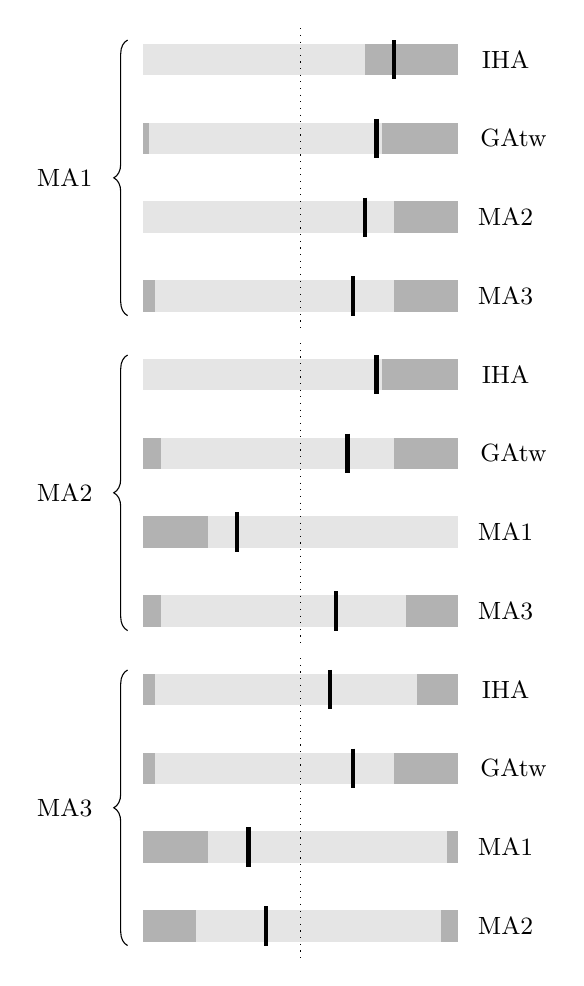
\begin{tikzpicture}
[help lines/.style={thin,draw=black!50},
 bar/.style={ultra thick},
 bad/.style={black, opacity=.3},
 good/.style={black, opacity=.3},
 eq/.style={black, opacity=.1},
 label/.style={font=\small},
 braces/.style={decorate,decoration={brace,amplitude=.5em},draw=black}]
\draw[braces] (-2.2, -3.25) -- (-2.2, .25);
\draw[braces] (-2.2, -7.25) -- (-2.2, -3.75);
\draw[braces] (-2.2, -11.25) -- (-2.2, -7.75);
\node[label] at (-3, -1.5) {MA1};
\node[label] at (-3, -5.5) {MA2};
\node[label] at (-3, -9.5) {MA3};
\node[label] at (+2.6, 0) {IHA};
\node[label] at (+2.7, -1) {GAtw};
\node[label] at (+2.6, -2) {MA2};
\node[label] at (+2.6, -3) {MA3};
\node[label] at (+2.6, -4) {IHA};
\node[label] at (+2.7, -5) {GAtw};
\node[label] at (+2.6, -6) {MA1};
\node[label] at (+2.6, -7) {MA3};
\node[label] at (+2.6, -8) {IHA};
\node[label] at (+2.7, -9) {GAtw};
\node[label] at (+2.6, -10) {MA1};
\node[label] at (+2.6, -11) {MA2};
%\draw[style=help lines] (-2.0, 0) -- (+2.0, 0);
%\draw[style=help lines] (-2.0, -1) -- (+2.0, -1);
%\draw[style=help lines] (-2.0, -2) -- (+2.0, -2);
%\draw[style=help lines] (-2.0, -3) -- (+2.0, -3);
%\draw[style=help lines] (-2.0, -4) -- (+2.0, -4);
%\draw[style=help lines] (-2.0, -5) -- (+2.0, -5);
%\draw[style=help lines] (-2.0, -6) -- (+2.0, -6);
%\draw[style=help lines] (-2.0, -7) -- (+2.0, -7);
%\draw[style=help lines] (-2.0, -8) -- (+2.0, -8);
%\draw[style=help lines] (-2.0, -9) -- (+2.0, -9);
%\draw[style=help lines] (-2.0, -10) -- (+2.0, -10);
%\draw[style=help lines] (-2.0, -11) -- (+2.0, -11);
\draw[dotted] (0, 0.4) -- (0, -3.4);
\draw[dotted] (0, -3.6) -- (0, -7.4);
\draw[dotted] (0, -7.6) -- (0, -11.4);
% MA1/IHA
   \fill[style=eq] (-2,.2) rectangle (0.814,-.2);
   \fill[style=bad] (0.814,.2) rectangle (2,-.2);
   \draw[style=bar] (+1.186, .25) -- (+1.186, -.25);
% MA1/GAtw
   \fill[style=good] (-2,-0.8) rectangle (-1.926,-1.2);
   \fill[style=eq] (-1.926,-0.8) rectangle (1.037,-1.2);
   \fill[style=bad] (1.037,-0.8) rectangle (2,-1.2);
   \draw[style=bar] (+0.963, -0.75) -- (+0.963, -1.25);
% MA1/MA2
   \fill[style=eq] (-2,-1.8) rectangle (1.185,-2.2);
   \fill[style=bad] (1.185,-1.8) rectangle (2,-2.2);
   \draw[style=bar] (+0.814, -1.75) -- (+0.814, -2.25);
% MA1/MA3
   \fill[style=good] (-2,-2.8) rectangle (-1.852,-3.2);
   \fill[style=eq] (-1.852,-2.8) rectangle (1.185,-3.2);
   \fill[style=bad] (1.185,-2.8) rectangle (2,-3.2);
   \draw[style=bar] (+0.666, -2.75) -- (+0.666, -3.25);
% MA2/IHA
   \fill[style=eq] (-2,-3.8) rectangle (1.037,-4.2);
   \fill[style=bad] (1.037,-3.8) rectangle (2,-4.2);
   \draw[style=bar] (+0.963, -3.75) -- (+0.963, -4.25);
% MA2/GAtw
   \fill[style=good] (-2,-4.8) rectangle (-1.778,-5.2);
   \fill[style=eq] (-1.778,-4.8) rectangle (1.185,-5.2);
   \fill[style=bad] (1.185,-4.8) rectangle (2,-5.2);
   \draw[style=bar] (+0.593, -4.75) -- (+0.593, -5.25);
% MA2/MA1
   \fill[style=good] (-2,-5.8) rectangle (-1.185,-6.2);
   \fill[style=eq] (-1.185,-5.8) rectangle (2,-6.2);
   \draw[style=bar] (-0.814, -5.75) -- (-0.814, -6.25);
% MA2/MA3
   \fill[style=good] (-2,-6.8) rectangle (-1.778,-7.2);
   \fill[style=eq] (-1.778,-6.8) rectangle (1.334,-7.2);
   \fill[style=bad] (1.334,-6.8) rectangle (2,-7.2);
   \draw[style=bar] (+0.444, -6.75) -- (+0.444, -7.25);
% MA3/IHA
   \fill[style=good] (-2,-7.8) rectangle (-1.852,-8.2);
   \fill[style=eq] (-1.852,-7.8) rectangle (1.481,-8.2);
   \fill[style=bad] (1.481,-7.8) rectangle (2,-8.2);
   \draw[style=bar] (+0.370, -7.75) -- (+0.370, -8.25);
% MA3/GAtw
   \fill[style=good] (-2,-8.8) rectangle (-1.852,-9.2);
   \fill[style=eq] (-1.852,-8.8) rectangle (1.185,-9.2);
   \fill[style=bad] (1.185,-8.8) rectangle (2,-9.2);
   \draw[style=bar] (+0.666, -8.75) -- (+0.666, -9.25);
% MA3/MA1
   \fill[style=good] (-2,-9.8) rectangle (-1.185,-10.2);
   \fill[style=eq] (-1.185,-9.8) rectangle (1.852,-10.2);
   \fill[style=bad] (1.852,-9.8) rectangle (2,-10.2);
   \draw[style=bar] (-0.666, -9.75) -- (-0.666, -10.25);
% MA3/MA2
   \fill[style=good] (-2,-10.8) rectangle (-1.334,-11.2);
   \fill[style=eq] (-1.334,-10.8) rectangle (1.778,-11.2);
   \fill[style=bad] (1.778,-10.8) rectangle (2,-11.2);
   \draw[style=bar] (-0.444, -10.75) -- (-0.444, -11.25);
\end{tikzpicture}
\caption[Result of the comparisons]{Result of the comparisons on the validation instances. Dark areas represent instances where the respective side performs significantly better than the other (significance level $\alpha=\SI{5}{\percent}$). The remaining light areas in between represent instances where no performance difference could be identified. The verical black bars signify the result of the respective comparison}
   \label{fig:comparison-result}
\end{figure}



%\clearpage
%\section{Comparing Arithmetic Means of Normalized Treewidths}
 %\label{sec:results_arith}

%%As the instances are of different sizes, all algorithm's results have to be gathered using the same instances. Additionally, in order not to introduce any bias, the number of samples per instance has to be the same over all instances and algorithms. Furthermore, the results have to be normalized\Index{normalization}.

%To motivate treewidth\Index{normalization} normalization, consider two instances, instance $I_1$ with $1000$ vertices and instance $I_2$ with $100$ vertices, and two algorithms, $A$ and $B$. Assume the following results when $A$ and $B$ are applied to $I_1$ and $I_2$:
%\begin{align*}
   %A&:\quad \mathrm{tw}(I_1) = 110;\; \mathrm{tw}(I_2) = 40\\
   %B&:\quad \mathrm{tw}(I_1) = 140;\; \mathrm{tw}(I_2) = 10\;.
%\end{align*}
%Intuitively, algorithm $B$ performs better than $A$, for the \emph{relative difference in treewidth} is larger for $I_2$. The arithmetic mean, however, shows the two algorithms to perform equally well, at a score of $\frac{110 + 40}{2} = \frac{140 + 10}{2} = 75$. To mitigate this effect, the algorithm's results are normalized using the instance's number of vertices, which is a definite upper bound on the respective treewidth. The results change to
%\begin{align*}
   %A&:\quad \mathrm{score}(I_1) = \tfrac{110}{1000} = 0.110;\; \mathrm{score}(I_2) = \tfrac{40}{100} = 0.40;\; \Rightarrow \overline{\mathrm{score}_A} = 0.255\\
   %B&:\quad \mathrm{score}(I_2) = \tfrac{140}{1000} = 0.140;\; \mathrm{score}(I_2) = \tfrac{10}{100} = 0.10;\; \Rightarrow \overline{\mathrm{score}_B} = 0.12\;.
%\end{align*}
%Having a lower overall score, algorithm $B$ is shown to perform better than algorithm $A$.

%\pfbreak
%\TODO{results here}

%\section{Comparing Geometric Means of Normalized Treewidths}
 %\label{sec:results_geom}

 %In the previous Section, normalization has been used to allow for an performance-wise ordering of the algorithms that incorporates the instance's complexity in a simple way. This Section investigates on how using the geometric mean instead of the arithmetic mean changes the results. The motivation behind using the geometric mean is to lower the effect of the normalization non-linearily.

%\TODO{results here}

%\appendix
%\printglossaries
%\printbibliography
\end{document}
% vim: set ts=3 sts=3 sw=3 tw=0 et :
